\chapter{'വരവില' എന്ന നുകം രൂപമെടുക്കുന്നു}
\label{chapter5}

\begin{figure}[h]
\begin{center}
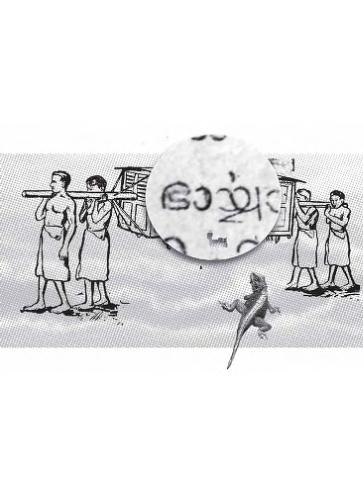
\includegraphics[width=0.5\textwidth,height=8cm]{Kulasthree_Chapter_five_pic01.jpg}
\end{center}
%\caption*{പുലയർ - കെ പി പത്മനാഭ മേനോൻ - വാള്യം 3, (1929), 1984}
\end{figure}

സ്ത്രീധനത്തെക്കുറിച്ച് വേവലാതിപ്പെടാത്ത കുടുംബങ്ങൾ ഇന്ന് കേരളത്തിൽ കുറവാണ്. എന്നാൽ ഈ സമ്പ്രദായം നാട്ടിലാകെ പടർന്നുപിടിച്ചത് അൽപകാലം മുമ്പുമാത്രമാണെന്നതാണ് വാസ്തവം. മാത്രമല്ല, ഇന്ന് 'സ്ത്രീക്കു നൽകുന്ന ധന'മല്ല സ്ത്രീധനം - 'വരനു നൽകുന്ന വില'യാണ്. വിവാഹസ്ഥിരതയെക്കുറിച്ചും കുടുംബത്തിൽ ഭർത്താവിന്റെ അധികാരങ്ങളെക്കുറിച്ചുമുള്ള ധാരണകളിലുമുണ്ടായ മാറ്റങ്ങളിൽനിന്നാണ് സ്ത്രീധനമേർപ്പാട് രൂപപ്പെട്ടത്. സാമൂഹ്യമാറ്റത്തിനിടയിൽ ഉയർന്നുവന്ന തിന്മയാണ് സ്ത്രീധനമെന്നു തിരിച്ചറിയുമ്പോൾ സാമൂഹ്യമാറ്റത്തിലൂടെ അതിനെ ഇല്ലായ്മചെയ്യാനാകുമെന്നതിനെക്കുറിച്ചുള്ള ആത്മവിശ്വാസവും വർദ്ധിക്കുന്നു.

\section{'സ്ത്രീധനം' അല്ല!}
\label{ch5sec1}

\paragraph{}തുടക്കത്തിൽത്തന്നെ പറയാം, കേരളത്തിൽ വിവാഹങ്ങളോടനുബന്ധിച്ച് നടക്കുന്ന കൊടുക്കൽവാങ്ങലിന് 'സ്ത്രീധനം' എന്ന പേർ യോജിക്കില്ല. കല്യാണവേളയിൽ വധുവിന് സ്വന്തം കുടുംബം നൽകുന്ന സമ്മാനമാണ് 'സ്ത്രീധനം'. അതവൾക്ക് നേരിട്ടവകാശപ്പെട്ടതും സ്വന്തമായി കൈകാര്യം ചെയ്യാവുന്നതുമായ മുതലാണ്. എന്തെങ്കിലും കാരണവശാൽ അവൾക്ക് വിവാഹബന്ധം ഒഴിയേണ്ടിവന്നാൽ സ്ത്രീധനം മടക്കിക്കൊടുക്കാൻ ഭർത്താവിന്റെ വീട്ടുകാർ ബാദ്ധ്യസ്ഥരുമാണ്. പക്ഷേ കേരളത്തിൽ ഇന്നു നിലവിലുള്ള രീതി ഇതല്ല; അത് 'വരവില'യാണ് - വധുവിന്റെ വീട്ടുകാർ വരന്റെ 'യോഗ്യത'യനുസരിച്ച് അയാൾക്കു നൽകുന്ന ധനം - വരന്റെ 'യോഗ്യത'യനുസരിച്ച് അത് കൂടിയും കുറഞ്ഞുമിരിക്കും. വധുവിന്റെ 'യോഗ്യത'യും പരിഗണിക്കാറുണ്ടെങ്കിലും അതിനു താരതമ്യേന പ്രാധാന്യം കുറവാണ്.

\paragraph{}ഇന്ന് കേരളത്തിലെ താണ-ഇടത്തരം കുടുംബങ്ങളെ ദാരിദ്യ്രത്തിലേക്കു വലിച്ചിഴക്കുന്ന പ്രധാന കാരണങ്ങൾ രണ്ടാണ്. ഒന്ന് ചെലവേറിയ ചികിത്സ ആവശ്യമായിവരുന്ന രോഗങ്ങൾ; രണ്ട്, പെൺകുട്ടികളെ എന്തു നഷ്ടവും സഹിച്ച് 'അയയ്ക്കണം' എന്ന ചിന്ത. ആദ്യത്തേതിനുമേൽ നമുക്കധികം നിയന്ത്രണം ഒരുപക്ഷേ ഇല്ലായിരിക്കാം. രണ്ടാമത്തേത് നാംതന്നെ വരുത്തിവയ്ക്കുന്നതാണ്. ആൺകുട്ടികളെപ്പോലെയോ അവരെക്കാൾ മെച്ചമായോ പഠിക്കാനും ജോലിചെയ്യാനും സമ്പാദിക്കാനും പെൺകുട്ടികൾക്കു കഴിയുമെന്ന് ഇന്നു നമുക്കറിയാം. പഠിത്തം, ജോലി, ഇവയിലേക്കു കടക്കാൻ പെൺകുട്ടികളെ നാം പ്രാത്സാഹിപ്പിക്കുന്നുമുണ്ട്. എന്നാൽ ഇതിലൊക്കെ അധികമാണ് പെൺകുട്ടികളെ വിവാഹം കഴിപ്പിക്കാനുള്ള പരിശ്രമം! പഠിച്ചുവളർന്ന പെൺകുട്ടി ആത്മാഭിമാനമുള്ള, മുതിർന്ന, ഒരു വ്യക്തിയാണെന്ന കാര്യത്തെപ്പോലും അവഗണിച്ചുകൊണ്ട് ഏതുവിധേനയും ഒരു വരനെക്കണ്ടെത്താൻ മാതാപിതാക്കന്മാർ ശ്രമിക്കും. ഒടുവിൽ വലിയ വിലകൊടുത്ത് ഒരാളെ കൊണ്ടുവരും. അതും ഒരു ഭാഗ്യപരീക്ഷണംമാത്രമാണ്. നന്നായില്ലെങ്കിൽ 'അവളുടെ തലയിലെഴുത്ത്' എന്ന് ദീർഘമായി നിശ്വസിക്കും; ആ അദ്ധ്യായം അടയ്ക്കും. പിന്നെ ആ സാധുപെൺകുട്ടിയുടെ നശിച്ചുപോയ ജീവിതം അവളുടെമാത്രം തലവേദനയാണ്.


\captionof{mybox}{കേരളത്തിലെ മിഷണറിസഭകൾ}
\label{ch5box1} % place the caption
\begin{tcolorbox}[%
 breakable, % make the box breakable
  arc=0mm, 
  left=1pt, right = 1pt, 
  boxrule=0mm,
  colback = {blue!10}, % since shadow-gray was not defined
] 


ചർച്ച് മിഷണറി സൊസൈറ്റി (CMS), ലണ്ടൻ മിഷണറി സൊസൈറ്റി (LMS), ബാസൽ മിഷൻ (Basel Mission) എന്നീ മൂന്നു സഭകളാണ് 19-ാം നൂറ്റാണ്ടുമുതൽ കേരളത്തിൽ പ്രേഷിതവേലയിൽ ഏർപ്പെട്ടത്. ഇവയിൽ ആദ്യത്തെ രണ്ട് സഭകൾ കേരളത്തിന്റെ തെക്കൻഭാഗങ്ങളിലും ബാസൽമിഷൻ വടക്കൻ കേരളത്തിലും പ്രവർത്തിച്ചു. 19-ാം നൂറ്റാണ്ടിൽ തിരുവിതാംകൂറിൽ ബ്രിട്ടിഷ് അധികാരത്തിന് അടിസ്ഥാനമിട്ട കേണൽ മൺറോയുടെ ഒത്താശയോടെയാണ് മിഷണറിപ്രവർത്തകർ ഈ നാട്ടിൽ ചുവടുറപ്പിച്ചത്. എന്നാൽ മതംമാറ്റുക എന്ന ഒരൊറ്റ ജോലിമാത്രമല്ല മിഷണറിമാർ ചെയ്തത്. ജാതിവ്യത്യാസങ്ങൾക്കപ്പുറത്ത് എല്ലാവർക്കും വിദ്യാഭ്യാസം നൽകിയിരുന്ന വിദ്യാലയങ്ങൾ ഈ നാട്ടിലാരംഭിച്ചത് അവരാണ്. കീഴാളർക്ക് വിദ്യയുടെ വെളിച്ചം എത്തിച്ചുകൊടുക്കുകവഴി നിലവിലുണ്ടായിരുന്ന ജാത്യാചാരത്തിലെ അനീതിയെയും അക്രമത്തെയും പ്രത്യക്ഷത്തിലെതിർക്കാനുള്ള ധൈര്യവും അവർ പകർന്നു. 1850കൾവരെ തെക്കൻ തിരുവിതാംകൂറിലെ നാടാന്മാർ ഉന്നതജാതിക്കാർക്കെതിരെ നടത്തിയ മാറുമറയ്ക്കൽ സമരത്തിന് ഉറച്ച പിന്തുണ നൽകിയത് LMS പാതിരിമാരായിരുന്നു. എല്ലാ ജാതിമതക്കാരും ഒന്നിച്ചു പഠിച്ച, ഉന്നതനിലവാരം പുലർത്തിയ, നിരവധി സ്കൂളുകളും കലാലയങ്ങളും അവർ സ്ഥാപിക്കുകയുണ്ടായി. വടക്ക് ബാസൽമിഷനാകട്ടെ, പല പുതിയ തൊഴിലുകളും ജനങ്ങളെ പരിശീലിപ്പിച്ചു. മലയാളഭാഷയ്ക്കും കനത്ത സംഭാവനകൾ മിഷണറിമാരിൽനിന്നുണ്ടായിട്ടുണ്ട്. ഹെർമ്മൻ ഗുണ്ടർട്ട്, ബെഞ്ചമിൻ ബെയ്ലി എന്നീ നാമങ്ങൾ മലയാളഭാഷാചരിത്രത്തിൽ തിളങ്ങിനിൽക്കുന്നവയാണ്.

\end{tcolorbox}

\paragraph{}എന്നാൽ പഴയകാലത്ത് സ്ത്രീധനം കൊടുക്കുന്നവർക്ക് വിവാഹബന്ധം ഒഴിഞ്ഞാൽ അതു മുഴുവനായോ ഭാഗികമായോ മടക്കിക്കിട്ടാനുള്ള സംവിധാനം പല സമുദായങ്ങളിലുമുണ്ടായിരുന്നു. വിവാഹസമയത്ത് കിട്ടുന്ന സമ്മാനങ്ങളുടെ കണക്ക് കൃത്യമായി എടുത്തുവയ്ക്കുന്ന രീതി ഇന്നും പല സമുദായങ്ങളിലുമുണ്ട്. ഈ പഴുതുകളെല്ലാം ഇരുപതാംനൂറ്റാണ്ടിൽ ചുരുങ്ങുകയാണുണ്ടായത്. വരവിലയുടെ സ്വാധീനം വളരുംതോറും ഇന്ന് നിലവിലുള്ളവയുടെ ആയുസ്സു കുറയുമെന്നു തീർച്ചയാണ്. 20-ാംനൂറ്റാണ്ടിന്റെ പ്രത്യേകത അതുമാത്രമല്ല. മുമ്പ് സ്ത്രീധനസമ്പ്രദായം തീരെ പതിവില്ലായിരുന്ന സമുദായങ്ങളിലേക്ക് വരവില കടന്നുകയറിയതാണ് 20-ാം നൂറ്റാണ്ടിന്റെ സവിശേഷത.



\paragraph{}'വരവില'യുടെ വരവിനെക്കുറിച്ചാണ് ഈ അദ്ധ്യായം. ഇത്തിൾക്കണ്ണിപോലെ എല്ലാ സമുദായങ്ങളിലും - പണക്കാർ, പാവപ്പെട്ടവർ എന്ന വ്യത്യാസമൊന്നും കൂടാതെ - കയറിപ്പറ്റിയ ഈ ഏർപ്പാട് കേരളത്തിലെ മൊത്തം സ്ത്രീകളും നേരിടുന്ന വിപത്തായിത്തീർന്നിരിക്കുന്നുവെന്നത് പരിഗണിച്ചാണ് അതിനിവിടെ ഇത്രയും പ്രാധാന്യം കല്പിച്ചിരിക്കുന്നത്. ചില ചെറിയ ആദിവാസിഗോത്രങ്ങളിലൊഴിച്ച് മറ്റെല്ലായിടത്തും 'വരവില' പടർന്നുപിടിച്ചിരിക്കുന്നു. മുമ്പാണെങ്കിൽ മലയാളബ്രാഹ്മണർ, ക്രിസ്ത്യാനികൾ തുടങ്ങിയ മക്കത്തായ സമുദായങ്ങൾക്കിടയിലായിരുന്നു സ്ത്രീധനമേർപ്പാട് പൂർണ്ണരീതിയിൽ നിലനിന്നിരുന്നത്. എന്നാൽ 19-ാം നൂറ്റാണ്ടിൽപ്പോലും 'സ്ത്രീധനം' 'വരവില' തന്നെയായിരുന്നില്ലേ എന്നു സംശയിക്കാൻ വകയുണ്ട്. 1822ൽ തിരുവിതാംകൂറിലെ റാണി ഗൗരിപാർവ്വതീഭായി ഒപ്പുവച്ച ഒരു ഉത്തരവുപ്രകാരം ഇവിടത്തെ നമ്പൂതിരി-പോറ്റി സമുദായങ്ങളുടെ സ്ത്രീധനമേർപ്പാടിനുമേൽ നിയന്ത്രണമേർപ്പെടുത്താൻ സർക്കാർ ശ്രമിച്ചതായി കാണുന്നു. ക്രമാതീതമായി വർദ്ധിച്ച സ്ത്രീധനത്തുകമൂലം ബ്രാഹ്മണസ്വത്തുക്കൾ നശിക്കുന്നെന്നും അവിവാഹിതകളായിനിൽക്കുന്ന സ്ത്രീകൾക്ക് പലവിധ ദോഷങ്ങളും ഉണ്ടാകുന്നുവെന്നും ഉത്തരവിൽ പറയുന്നു. സ്ത്രീധനത്തുക നിശ്ചയിച്ചതിനുപുറമെ 14 വയസ്സിലധികം പ്രായമായ കന്യകമാരുടെ വിവാഹം ഉടൻതന്നെ നടത്തിക്കൊള്ളണമെന്നും ഉത്തരവിൽ പറഞ്ഞിരിക്കുന്നു! വരന്മാരുടെ വിലയായിരുന്നു ഇവിടെ സ്ത്രീധനം എന്നു കരുതാൻ കാരണമുണ്ട്; ബ്രഹ്മസ്വങ്ങൾ നശിക്കാൻമാത്രം ഉയർച്ചയാണ്. തുകയിലുണ്ടായത്! ഇതുപോലെ കോട്ടയത്തെ സുറിയാനിക്രിസ്ത്യാനികളുടെ ഗൃഹജീവിതവുമായി തനിക്കുണ്ടായിരുന്ന പരിചയത്തെ അടിസ്ഥാനമാക്കി സി.എം.എസ്. മിഷണറിസഭയിൽ പ്രവർത്തിച്ചിരുന്ന മിഷണറിയായിരുന്ന കോളിൻസ് മദാമ്മ 1877ൽ പ്രസിദ്ധീകരിച്ച ഘാതകവധം എന്ന നോവലിലും 'സ്ത്രീധനം' 'വരവില'യായിരുന്നുവെന്ന് സൂചനയുണ്ട്. പുരുഷന്റെ യോഗ്യതകൾക്ക് കൊടുത്ത അമിത പ്രാധാന്യവും സ്ത്രീയുടെ യോഗ്യതകളെ ഇടിച്ചുതാഴ്ത്താനുമുള്ള പ്രവണതയും ഈ നോവലിൽ വിമർശിക്കപ്പെടുന്നു. 'നല്ല കുടുംബ'മെന്ന യോഗ്യതയുള്ള വരനെ തന്റെ മകൾക്കു കിട്ടണമെങ്കിൽ ഒത്തിരി നിലം പുരയിടങ്ങൾ സമ്പാദിച്ചുകൂട്ടിയേ പറ്റൂ എന്നു വിശ്വസിച്ച കോശീകുര്യൻ എന്നയാളുടെ മനസ്സിനെ മകളായ മറിയം മാറ്റിയെടുത്തതിന്റെ കഥയാണ് ഘാതകവധം പറയുന്നത്.


\begin{figure}[h]
\begin{center}
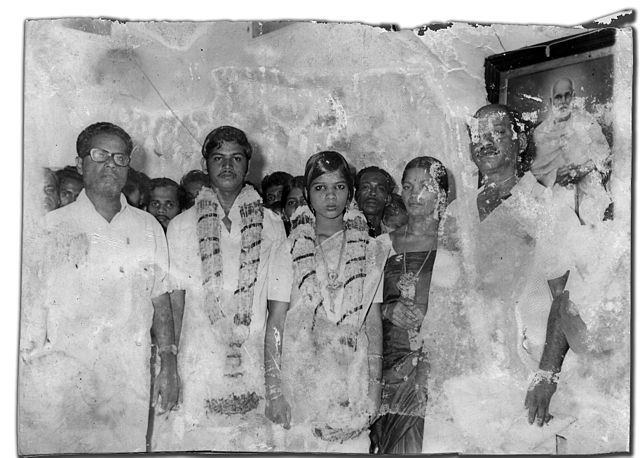
\includegraphics[width=\textwidth,height=8cm]{Kulasthree_Chapter_five_pic02.jpg}
\end{center}
%\caption*{പുലയർ - കെ പി പത്മനാഭ മേനോൻ - വാള്യം 3, (1929), 1984}
\end{figure}

\section{വരവില മാന്യമാകുന്നു}
\label{ch5sec2}
\paragraph{}
അമ്മവഴിക്ക് സ്വത്തവകാശം കണക്കാക്കിയിരുന്ന മരുമക്കത്തായ സമുദായങ്ങളിൽ വരവിലയ്ക്ക് അനുകൂലമായ വിവാഹസമ്പ്രദായമല്ല നിലനിന്നിരുന്നത്. സ്ത്രീക്ക് സ്വന്തം കുടുംബവുമായുള്ള ബന്ധം ഈ സമുദായങ്ങളിൽ വളരെ ശക്തമായിരുന്നു. ഭർത്താവിന്റെ വീട്ടിലാണ് താമസമെങ്കിലും ജനിച്ചവീട്ടിൽനിന്ന് സ്ത്രീ ഒരിക്കലും അകന്നുപോയിരുന്നില്ല. പിറന്നകുടുംബത്തിൽ സ്ത്രീക്കുള്ള ധനപരവും ധാർമ്മികവുമായ അവകാശങ്ങൾ വിവാഹത്തിനുശേഷവും നിലനിന്നുവെന്ന് സാരം. രണ്ടാമതായി, 'മുറച്ചെറുക്ക'നെയോ 'മുറപ്പെണ്ണി'നെയോ (അമ്മാവന്റെ മകൻ, മകൾ അങ്ങനെയുള്ളവരെ) വിവാഹംചെയ്യുന്ന രീതി ഇക്കൂട്ടർക്കിടയിൽ നിലവിലുണ്ടായിരുന്നതുകൊണ്ട് പലപ്പോഴും കല്യാണംകഴിക്കുന്ന പുരുഷൻ അന്യനായിരുന്നില്ല. തന്നെയുമല്ല, വിവാഹമോചനവും വിധവാവിവാഹവും സാധാരണകാര്യങ്ങളായി അംഗീകരിക്കപ്പെട്ടിരുന്നു. ഭാര്യയുടെ സംരക്ഷണത്തിന്റെ ചുമതല അധികവും അവളുടെ സ്വന്തം വീടിനുതന്നെയായിരുന്നതുകൊണ്ട് വിവാഹമോചനംമൂലം സ്ത്രീ തകർന്നുപോകുന്ന ഇന്നത്തെയവസ്ഥ ഉണ്ടായിരുന്നില്ല. കീഴ്ജാതിക്കാർക്കിടയിലാകട്ടെ, വിവാഹസമയത്ത് ചെറുക്കൻവീട്ടുകാർ പെൺവീട്ടുകാർക്ക് 'പെൺപണം' കാഴ്ചവയ്ക്കുന്നരീതി 19-ാം നൂറ്റാണ്ടിലുണ്ടായിരുന്നു. പരമ്പരാഗത മരുമക്കത്തായ കുടുംബങ്ങളിലെ സ്ത്രീകൾ എല്ലാവിധത്തിലും സ്വതന്ത്രകളായിരുന്നു എന്നല്ല പറഞ്ഞുവരുന്നത്. അമ്മാവന്മാരുടെയും ആങ്ങളമാരുടെയും വാക്കിനു കീഴ്വഴങ്ങിയാണ് സ്ത്രീകൾ കഴിഞ്ഞത്; പ്രായമേറിയ സ്ത്രീകൾക്ക്, വിശേഷിച്ച് അമ്മമാർക്ക്, പക്ഷേ, വളരെ മാന്യമായ സ്ഥാനവും കുടുംബത്തിന്റെ സ്വത്തുക്കൾ, പണമിടപാടുകൾ, വരുമാനം എന്നിവയെക്കുറിച്ചുള്ള തീരുമാനങ്ങളിൽ വലിയ പങ്കുമുണ്ടായിരുന്നു. മറ്റൊരുവിധത്തിൽപ്പറഞ്ഞാൽ, ഇന്നത്തെപ്പോലെ 'സ്നേഹത്തിന്റെ അധികാരം' മാത്രമായിരുന്നില്ല അമ്മമാരുടേത്. മലബാറിൽ 19-ാം നൂറ്റാണ്ടിന്റെ അവസാനകാലത്തും 20-ാം നൂറ്റാണ്ടിന്റെ തുടക്കത്തിലും ഗവേഷണം നടത്തിയ എഫ്. ഫാസറ്റ് (F. Fawcett) എന്ന നരവംശശാസ്ത്രജ്ഞൻ തന്റെ Nayars of Malabar (1901) എന്ന പുസ്തകത്തിൽ ഇവിടെ നിലവിലുണ്ടായിരുന്ന 'സംബന്ധവ്യവസ്ഥ'യെക്കുറിച്ച് ഇങ്ങനെയാണ് നിരീക്ഷിച്ചത്:


\begin{quotation}
എല്ലാ ലൈംഗികകാര്യങ്ങളിലും സ്ത്രീകൾക്കും പുരുഷന്മാർക്കും തുല്യസ്വാതന്ത്ര്യം അനുവദിക്കുന്നുവെന്നത് മരുമക്കത്തായവ്യവസ്ഥയുടെ അപൂർവ്വഗുണങ്ങളിലൊന്നുതന്നെ. ഒറ്റരാത്രിമാത്രമേ ഒന്നിച്ചു കഴിഞ്ഞുള്ളു എന്നാലും ഇരുകൂട്ടർക്കും പിരിഞ്ഞുപോകാൻ അനുവാദമുണ്ട്. ലൈംഗികതാത്പര്യം ഇല്ലാതിരിക്കുകയോ മറ്റുവിധത്തിലുള്ള മനഃപൊരുത്തം നഷ്ടമാവുകയോ ചെയ്താൽ ഇരുകൂട്ടർക്കും ബന്ധം വേർപെടുത്തി മറ്റുബന്ധങ്ങളിൽ ഏർപ്പെടാനുള്ള സ്വാതന്ത്ര്യമുണ്ടായിരുന്നു. ഇത് നിത്യവും ബന്ധം പിരിയാനുള്ള പ്രവണതയിൽ കലാശിക്കില്ലേ എന്ന സംശയമുണ്ടാകിനിടയുള്ളതുകൊണ്ട്, അത്തരത്തിലുള്ള യാതൊന്നും ഉണ്ടാവില്ലെന്നകാര്യം ഇവിടെ എടുത്തുപറയട്ടെ. വെറുതെയുള്ള വിവാഹമോചനം അപൂർവ്വമാണ്. സ്ഥിരവിവാഹമാണ് പതിവുരീതി. തറവാട്ടുസ്വത്ത് സ്ത്രീകളെയും അവരുടെ സന്തതികളെയും സംരക്ഷിക്കാനായി നീക്കിവയ്ക്കുന്ന രീതിയാണ് ഈ സമ്പ്രദായത്തിന്റെ അടിത്തറ എന്നു തോന്നുന്നു.
\flushright{(Nayars of Malabar, New Delhi. 1985, പുറം 236-37)}
\end{quotation}

\captionof{mybox}{ 'താലികെട്ടി അമ്മയായി'}
\label{ch5box2} % place the caption
\begin{tcolorbox}[%
 breakable, % make the box breakable
  arc=0mm, 
  left=1pt, right = 1pt, 
  boxrule=0mm,
  colback = {blue!10}, % since shadow-gray was not defined
] 

മരുമക്കത്തായികൾക്കിടയിൽ വിവാഹച്ചടങ്ങിനെക്കാളധികം പ്രാധാന്യം 'താലികെട്ടുകല്യാണം' എന്ന ചടങ്ങിനായിരുന്നു. മാസമുറയെത്തുംമുമ്പ് പെൺകുട്ടികളെ ഏതെങ്കിലും ബ്രാഹ്മണനെക്കൊണ്ടോ സമുദായത്തിലെതന്നെ പ്രമുഖരായവരെക്കൊണ്ടോ താലികെട്ടിക്കുന്ന ചടങ്ങായിരുന്നു നായന്മാർക്കിടയിലുണ്ടായിരുന്നത്. ഇതുകൊണ്ട് പെൺകുട്ടി അയാളുടെ ഭാര്യയായി എന്നർത്ഥമാകുന്നില്ല - ബാല്യത്തിൽനിന്ന് യൗവ്വനത്തിലേക്ക് അവൾ കടന്നുവെന്ന് പ്രഖ്യാപിക്കുന്ന ചടങ്ങുമാത്രമായിരുന്നു ഇത്. എന്നാൽ വളരെ നീണ്ടതും ചിലവേറിയതുമായ ആഘോഷമായിരുന്നതുകൊണ്ട് തറവാട്ടിൽ ആ പ്രായത്തിനടുത്തെത്തിയ പെൺകുട്ടികളുടെ താലികെട്ടുകല്യാണം ഒരുമിച്ചുനടത്തുന്ന രീതി പതിവായിരുന്നു. താലികെട്ടിക്കഴിഞ്ഞ പെൺകുട്ടി 'അമ്മയായി' എന്നായിരുന്നു ചൊല്ല്. മക്കത്തായികളായ ഈഴവർക്കിടയിൽ താലികെട്ട് നിർവ്വഹിച്ചിരുന്നത് അന്യപുരുഷന്മാരായിരുന്നില്ല; ഏതെങ്കിലും സ്ത്രീയായിരുന്നു അത് നിർവ്വഹിച്ചിരുന്നത്. സാമ്പത്തികസ്ഥിതി ഇല്ലാത്ത കുടുംബങ്ങൾ അതു ചെറിയതോതിൽ നടത്തിയിരുന്നു- പെൺകുട്ടിയുടെ അമ്മതന്നെ താലികെട്ടുകയോ ഒരു ബൊമ്മയെ അടുത്തിരുത്തിയശേഷം ഏതെങ്കിലും സ്ത്രീകളായ ബന്ധുക്കൾ താലികെട്ടുകയോ ചെയ്യുന്ന രീതികൾ നിലവിൽവന്നു. മാസമുറയാകുന്ന അവസരത്തെ ആഘോഷപൂർവ്വം കൊണ്ടാടുന്ന 'തിരണ്ടുകുളി' എന്ന ചടങ്ങും മക്കത്തായ-മരുമക്കത്തായ കുടുംബങ്ങളിൽ നടത്തിയിരുന്നു.
\paragraph{}

20-ാം നൂറ്റാണ്ടിന്റെ ആരംഭത്തിൽത്തന്നെ സമുദായപരിഷ്ക്കർത്താക്കൾ 'കെട്ടുകല്യാണ'ത്തെ രൂക്ഷമായി വിമർശിച്ചുതുടങ്ങി. അത് 'അസന്മാർഗ്ഗിക'മാണ്, അത് ബ്രാഹ്മണരോട് വിധേയത്വംകാട്ടുന്നു, ഭാരിച്ച ചിലവിനിടയാക്കുന്നു മുതലായ വിമർശനങ്ങൾ ഉയർന്നുവന്നു. 'കെട്ടുകല്യാണം' അവസാനിപ്പിക്കുന്നതിൽ അവർ വിജയിക്കുകയും ചെയ്തു. എന്നാൽ ഇന്നത്തെക്കാലത്ത് നമ്മുടെ നാട്ടിൽ നടന്നുവരുന്ന, ഭാരിച്ച ചിലവുവരുന്ന വിവാഹാഭാസങ്ങളെ എതിർക്കാനുള്ള ശക്തി പഴയ സമുദായപരിഷ്ക്കർത്താക്കളുടെ പിന്മുറക്കാർക്കില്ലെന്നതാണ് കൗതുകകരമായ കാര്യം!


\end{tcolorbox}

\paragraph{}തറവാട്ടിലെ കാരണവരും മൂത്തവരും ചേർന്നുറപ്പിച്ചിരുന്ന വിവാഹങ്ങളിൽ ഫാസറ്റ് വിവരിക്കുംപ്രകാരമുള്ള സ്വാതന്ത്ര്യം ഉണ്ടായിരുന്നോ എന്നു സംശയമാണ്. എന്നാൽ, ഇങ്ങനെ സ്ത്രീയോടന്വേഷിക്കാതെ ഉറപ്പിക്കുന്ന ബന്ധങ്ങളിൽപ്പോലും അവൾ ഭർത്താവിന്റെയോ ഭർതൃകുടുംബത്തിന്റെയോ പൂർണ്ണവരുതിയിൽ വന്നിരുന്നില്ല. സ്വന്തം തറവാട്ടിൽ അവൾക്കുള്ള സ്ഥാനം അതുമൂലം നഷ്ടമായിരുന്നില്ല. അമ്മാവന്മാരും ആങ്ങളമാരും അനീതി പ്രവർത്തിക്കുമ്പോൾ ചോദ്യംചെയ്യാനുള്ള ധൈര്യം പല സ്ത്രീകൾക്കും ഉണ്ടായിരുന്നില്ലെന്ന് അക്കാലത്തു ജീവിച്ചിരുന്ന പല വ്യക്തികളുടെയും ആത്മകഥകൾ വെളിവാക്കുന്നുണ്ട്. എങ്കിൽപ്പോലും സ്വന്തം കുടുംബത്തിൽ സഹോദരിക്കുള്ള അടിസ്ഥാനാവകാശത്തെ ഇല്ലാതാക്കാൻ എത്ര പ്രതാപിയായ സഹോദരനും എളുപ്പത്തിൽ സാധിക്കുമായിരന്നില്ല. എങ്കിലും ജാതിവ്യവസ്ഥയ്ക്കുള്ളിൽ നിലവിലുണ്ടായിരുന്ന വിലക്കുകളെ അതിലംഘിച്ച സ്ത്രീകൾ ജാതിയിൽനിന്നുതന്നെ പുറന്തള്ളപ്പെട്ടിരുന്നു. അതോടെ കുടുംബാവകാശങ്ങളും അവർക്കു നഷ്ടമായിരുന്നു.

\captionof{mybox}{മലബാർ മരുമക്കത്തായ കമ്മീഷൻ}
\label{ch5box2} % place the caption
\begin{tcolorbox}[%
 breakable, % make the box breakable
  arc=0mm, 
  left=1pt, right = 1pt, 
  boxrule=0mm,
  colback = {blue!10}, % since shadow-gray was not defined
] 

\paragraph{}മലബാറിലെ വിവാഹനിയമനിർമ്മാണത്തിന്റെ ആവശ്യകതയെക്കുറിച്ചു വിലയിരുത്താൻ 1890ൽ മദ്രാസ് സർക്കാർ നിയമിച്ച ഒരു കമ്മിഷനായിരുന്നു ഇത്. മലബാറിലെ മരുമക്കത്തായികളായ ഹിന്ദുക്കളുടെ അഭിപ്രായമാരായാനും 1887ൽ സി. ശങ്കരൻനായർ എന്ന നായർസമുദായപ്രമാണി തയ്യാറാക്കിയ മലബാർ വിവാഹനിയമം (Madras Marriage Bill) എത്രകണ്ട് പ്രയോജനപ്രദമാണെന്ന് വിലയിരുത്താനും കമ്മിഷൻ ശ്രമിച്ചു. മരുമക്കത്തായികളുടെ ഇടയിലെ വിവാഹം 'വിവാഹ'മല്ലെന്ന് ആധുനികവിദ്യാഭ്യാസംനേടിയ പല ചെറുപ്പക്കാരും വാദിച്ചുതുടങ്ങിയതിനെത്തുടർന്നായിരുന്നു കമ്മിഷന്റെ രൂപീകരണം. കൂടുതൽ യാഥാസ്ഥിതികമായ ബ്രാഹ്മണവിവാഹമാതൃകയ്ക്കടുത്തുവരുന്ന രീതിയിൽ മരുമക്കത്തായവിവാഹരീതിയെ എങ്ങനെ പരിഷ്ക്കരിക്കാമെന്ന ചിന്തയായിരുന്നു നായർസമുദായപരിഷ്ക്കർത്താക്കളുടെയുള്ളിൽ. വിവാഹത്തിൽ സ്ത്രീപുരുഷന്മാരുടെ അവകാശങ്ങളെ നിജപ്പെടുത്തിയും വിവാഹമോചനത്തിന് നിയമപരമായ തടസ്സങ്ങൾ വരുത്തിയും 'പരിഷ്കൃതവിവാഹ'ത്തിലേക്ക് മരുമക്കത്തായികൾ കടക്കണമെന്നായിരുന്നു പരിഷ്ക്കാരികളുടെ അഭിപ്രായം. 1891ൽ മലബാറിലെ പലയിടങ്ങളിലുംവച്ച് കമ്മിഷനംഗങ്ങൾ തെളിവു ശേഖരിച്ചു. തെളിവു നൽകിയവരിൽ സ്ത്രീകൾ നന്നെ കുറവായിരുന്നു. കമ്മിഷൻ അംഗങ്ങൾ തമ്മിൽത്തന്നെ മലബാർ മരുമക്കത്തായവിവാഹരീതിയെപ്പറ്റി കാര്യമായ അഭിപ്രായവ്യത്യാസമുണ്ടായിരുന്നു. മരുമക്കത്തായവിവാഹം വെറും 'വെപ്പാട്ടിവ്യവസ്ഥ'യാണെന്ന വാദത്തോട് കമ്മിഷൻ അംഗമായിരുന്ന ഒ. ചന്തുമേനോൻ ശക്തമായി വിയോജിച്ചു. ശങ്കരൻനായർ തയ്യാറാക്കിയ ബില്ല് വിവാഹങ്ങൾ രജിസ്റ്റർ ചെയ്യാൻ താത്പര്യപ്പെടുന്നവർക്ക് അതിനുള്ള സൗകര്യം നൽകി. ഇത്തരം വിവാഹങ്ങൾ ആജീവനാന്തമുള്ള സാധുതയുള്ളവയും ഏകഭാര്യാവ്യവസ്ഥയ്ക്കു കീഴ്പ്പെട്ടവയും ആയിരിക്കണമെന്ന് ബിൽ നിഷ്ക്കർഷിച്ചു. തന്നെയുമല്ല, ഇപ്രകാരം രജിസ്റ്റർചെയ്ത വിവാഹങ്ങൾക്കുമാത്രമേ വിവാഹമോചനം, സ്വത്തുക്കളുടെ അനന്തരാവകാശം എന്നിവയെ സംബന്ധിച്ചുള്ള സിവിൽ അവകാശങ്ങൾ ബാധകമാകുമായിരുന്നുള്ളൂ. മരുമക്കത്തായകമ്മിഷന്റെ പ്രവർത്തനത്തിനിടയിൽ ഇതെല്ലാം മലബാറിൽ ചൂടേറിയ ചർച്ചാവിഷയമായി. നിയമം ആവശ്യമാണെന്ന തീരുമാനത്തിലാണ് കമ്മിഷൻ അംഗങ്ങളിൽ ഭൂരിഭാഗംപേരും എത്തിച്ചേർന്നത്; മരുമക്കത്തായത്തിൽ ശരിയായ വിവാഹനിയമമില്ലെന്ന് അവർ വാദിച്ചു. ചില തിരുത്തലുകളോടെ ശങ്കരൻനായരുടെ ബില്ല് സ്വീകരിക്കാവുന്നതാണെന്ന് കമ്മിഷൻ അഭിപ്രായപ്പെട്ടു. മരുമക്കത്തായസമ്പ്രദായത്തിനെതിരെ 19-ാം നൂറ്റാണ്ടുമുതൽ ആരംഭിച്ച നീക്കങ്ങളെ സ്ത്രീപക്ഷത്തുനിന്ന് വിലയിരുത്തുന്ന ചരിത്രപഠനങ്ങൾ ഇന്ന് ലഭ്യമാണ്. പ്രവീണാ കോടോത്ത്, ജി. അരുണിമ, കെ. ശാരദാമണി എന്നിവരുടെ കൃതികൾ ശ്രദ്ധിക്കുക ('കൂടുതൽ വായനയ്ക്ക്' എന്ന ഭാഗം നോക്കുക. \ref{chapter12}).
\end{tcolorbox}

\paragraph{}വിവാഹമോചനവും പുനർവിവാഹവും സാധാരണയായിരുന്നു. തിരുവിതാംകൂറിലെ റാണി ഗൗരി പാർവ്വതീഭായി മൂന്നു വിവാഹം കഴിച്ചിരുന്നു; അത് അന്നത്തെ മരുമക്കത്തായ സമുദായങ്ങളിലെ നടപ്പുരീതിയായിരുന്നു. മരുമക്കത്തായമെന്നാൽ 'നമ്പൂതിരി സംബന്ധം' - അതായത്, ജാതിശ്രേണിയിൽ ഉയർന്നജാതിയായ മലയാളബ്രാഹ്മണർ അതിൽ താഴെനിന്ന നായർ-അമ്പലവാസി സമുദായങ്ങളിലെ സ്ത്രീകളുമായി ഏർപ്പെട്ടിരുന്ന വിവാഹബന്ധം - ആയിരുന്നുവെന്ന ഒരു ധാരണ പൊതുവേയുണ്ട്. നമ്പൂതിരിസംബന്ധം 'അയഞ്ഞതോ' 'താത്കാലിക'മോ ആയിരുന്നുവെന്ന് പലരും പറഞ്ഞുകേൾക്കാറുണ്ട്. ഇപ്പറഞ്ഞത് അത്രയ്ക്കൊന്നും ശരിയല്ല എന്ന് നമ്പൂതിരിസംബന്ധത്തെക്കുറിച്ച് പഠിച്ച നരവംശശാസ്ത്രജ്ഞർ രേഖപ്പെടുത്തിയിട്ടുണ്ട്. അതുപോലെ ഇത്തരം ബന്ധങ്ങളിൽ ജീവിച്ച സ്ത്രീകൾ അധികവും ചൂഷണംചെയ്യപ്പെട്ടു എന്ന ധാരണയും തെറ്റാണെന്ന് ഈ പഠനങ്ങൾ വ്യക്തമാക്കുന്നു. വാസ്തവത്തിൽ 'മരുമക്കത്തായം' എന്നു നമ്മൾ പൊതുവെ പറയുന്നുണ്ടെങ്കിലും കേരളത്തിന്റെ പലഭാഗത്തും പല രീതിയിലുള്ള വിവാഹക്രമങ്ങളാണ് മരുമക്കത്തായസമുദായക്കാർ പിന്തുടർന്നുവന്നിരുന്നത്. തെക്കേമലബാർ - കൊച്ചീപ്രദേശങ്ങളിൽ നമ്പൂതിരിസംബന്ധം ധാരാളമുണ്ടായിരുന്നെങ്കിലും തിരുവിതാംകൂറിൽ പലയിടത്തും മുറച്ചെറുക്കനും മുറപ്പെണ്ണുമായുള്ള വിവാഹം വളരെ പ്രചാരത്തിലുണ്ടായിരുന്നു. തെക്കൻ പ്രദേശങ്ങളിൽ 'ബഹുഭർതൃത്വം' അല്ലെങ്കിൽ 'പാണ്ഡവാചാരം' എന്ന രീതിയും കണ്ടിരുന്നു. ഒരു സ്ത്രീക്ക് ഒരേസമയം പല ഭർത്താക്കന്മാർ ഉണ്ടായിരിക്കുന്നതാണ് 'ബഹുഭർതൃത്വം'; അവർ സഹോദരന്മാർകൂടിയാണെങ്കിൽ അതു 'പാണ്ഡവാചാരം'. വടക്കേ മലബാറിൽ സംബന്ധംകഴിഞ്ഞാൽ ഭാര്യ ഭർത്താവിന്റെ കുടുംബത്തിൽ പോയി താമസിക്കുന്നതായിരുന്നു പതിവ്. ഇതോടൊപ്പം സ്വന്തം വീടുമായുള്ള ബന്ധം അവർ നിലനിർത്തി. ഭർത്താവ് മരിക്കാനിടവന്നാൽ സ്വന്തം കുടുംബത്തിലേക്ക് മടങ്ങുകയും ചെയ്തു. തെക്കേ മലബാറിലാകട്ടെ, ഭാര്യ സ്വന്തം തറവാട്ടിൽത്തന്നെ താമസിക്കുകയും ഭർത്താവ് അവിടെച്ചെന്ന് അവരെ സന്ദർശിക്കുകയും ചെയ്യുന്ന രീതിയായിരുന്നു.

\paragraph{}ഇതുകൂടാതെ വിവാഹംനടത്തുന്ന രീതിയിലും വിവാഹബന്ധത്തിലും പല വ്യത്യാസങ്ങളും കണ്ടിരുന്നു. സമൂഹം അംഗീകരിച്ച ഒരു രീതിയല്ല, പല രീതികളായിരുന്നു ഉണ്ടായിരുന്നത്. ഇന്ന് ഇവിടെ വ്യാപകമായി അംഗീകരിക്കപ്പെടുന്ന 'പുടമുറി സംബന്ധം' അവയിൽ ഒരു രീതിമാത്രമായിരുന്നു. (താലികെട്ടുക എന്ന ചടങ്ങുകൂടി ഇതോടൊപ്പം ചേർത്താണ് ഇന്നിത് ആചരിക്കുന്നത്). കുറച്ചുകൂടി അയഞ്ഞ, എന്നാൽ സമൂഹത്തിന്റെ അംഗീകാരമുള്ള മറ്റു ചടങ്ങുകളുമുണ്ടായിരുന്നു. 'വീടാരം കയറുക' എന്ന ചടങ്ങ് ഒരുദാഹരണമാണ്. ഇതുപ്രകാരം പുടവ നൽകുന്ന ചടങ്ങോ വിസ്തരിച്ചുള്ള സദ്യയോ ഒന്നും നടത്തിയിരുന്നില്ല; പക്ഷേ, 'വീടാരംകയറി'യ ദമ്പതിമാരുടെ മക്കൾക്ക് സമൂഹത്തിന്റെ അംഗീകാരം ലഭിച്ചിരുന്നു. സാഹചര്യം ഒത്തുവരുമ്പോൾ 'വീടാരം കയറിയ'വർ പുടമുറി നടത്തുകയും ചെയ്തിരുന്നു. ഇരുപതു വർഷത്തിനുശേഷം പുടമുറി നടത്തിയ 'വീടാരം കയറിയ'വരെ തനിക്ക് പരിചയമുണ്ടെന്ന് പ്രശസ്ത സാഹിത്യകാരനും ആ കാലത്തെ മലബാറിലെ പൊതുരംഗത്തു പ്രസിദ്ധനുമായിരുന്ന ഒ. ചന്തുമേനോൻ മലബാർ മരുമക്കത്തായ കമ്മിഷന് (1891) തെളിവു നൽകി! ഇതിനുപുറമേ, 'കിടക്കോറക്കല്യാണം', 'കിടപ്പിന്റെ വട്ടം' എന്നിങ്ങനെയുള്ള കൂടുതൽ ലഘുവായ, എന്നാൽ സമൂഹം അംഗീകരിക്കുന്ന, ബന്ധങ്ങൾ നിലവിലുണ്ടായിരുന്നു. സമൂഹത്തിന്റെ അംഗീകാരമില്ലാത്ത ബന്ധങ്ങളെയാണ് 'രഹസ്യ'മെന്നോ 'സ്വകാര്യ'മെന്നോ വിളിച്ചിരുന്നത്. ഇന്നാകട്ടെ, 'കിടക്കോറക്കല്യാണവും', 'വീടാരംകയറലും' ഒന്നും നിലവിലില്ല; 'രഹസ്യ'ത്തിനും 'സ്വകാര്യ'ത്തിനും വലിയ കുറവൊന്നുമില്ല!


\begin{figure}[h]
\begin{center}
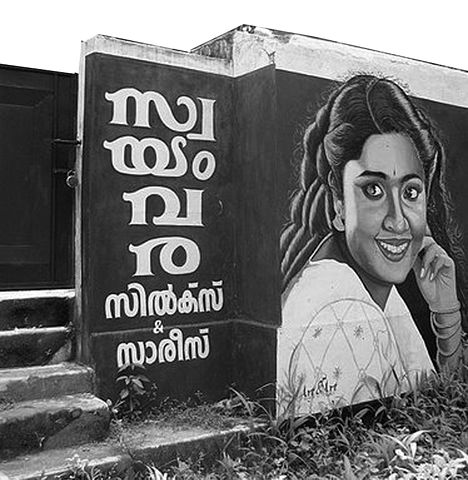
\includegraphics[width=\textwidth,height=8cm]{Kulasthree_Chapter_five_pic03.jpg}
\end{center}
%\caption*{പുലയർ - കെ പി പത്മനാഭ മേനോൻ - വാള്യം 3, (1929), 1984}
\end{figure}

\paragraph{}അതുപോലെ മരുമക്കത്തായക്കാരെല്ലാം നായന്മാരായിരുന്നില്ലെന്നും ഓർക്കണം. വടക്കേമലബാറിലെ തീയ്യർ, ഈഴവസമുദായത്തിലെ ചില വിഭാഗക്കാർ, മരുമക്കത്തായരീതി പിൻതുടർന്ന മാപ്പിളവിഭാഗക്കാർ, പുലയർ, മറ്റു കീഴാളജാതിക്കാർ, ഇവരെക്കൂടി എണ്ണിയിട്ടുവേണം മരുമക്കത്തായത്തെക്കുറിച്ചു പറയാൻ. ഇവരിൽ ആർക്കും നമ്പൂതിരിസംബന്ധം ഇല്ലായിരുന്നു; മേൽപ്പറഞ്ഞ പലവിധത്തിലുള്ള വിവാഹരീതികൾ ഇക്കൂട്ടരുടെയിടയിലും ഏകദേശം 20-ാം നൂറ്റാണ്ടിന്റെ പകുതിയോളവും ചിലയിടങ്ങളിൽ അതിനുശേഷവും നിലവിലുണ്ടായിരുന്നു.

\paragraph{}19-ാം നൂറ്റാണ്ടിന്റെ അവസാനഘട്ടത്തിൽ ഇംഗ്ലീഷ് വിദ്യാഭ്യാസം നേടിയ മരുമക്കത്തായികളിൽ പലർക്കും - ഇവർ അധികവും പുരുഷന്മാരായിരുന്നു - ഇത്തരം നടപ്പുരീതികളെക്കുറിച്ച് നാണക്കേടും അതൃപ്തിയും തോന്നിത്തുടങ്ങിയിരുന്നു. രണ്ടുതരം സ്വാധീനങ്ങളായിരുന്നു ഈ അഭിപ്രായത്തിനുപിന്നിൽ. ഒന്ന്, ആധുനികവിദ്യാഭ്യാസത്തിലൂടെ ഇന്ത്യയിലാകെ രൂപപ്പെട്ടുതുടങ്ങിയിരുന്ന പുതിയ മേൽജാതിസംസ്കാരത്തിന്റെ സ്വാധീനം. ബ്രാഹ്മണമൂല്യങ്ങൾക്ക് കണക്കിലധികം വില കല്പിക്കുകയും 'ഇന്ത്യൻസംസ്കൃതി'യുടെ അന്തഃസത്ത ബ്രാഹ്മണമൂല്യങ്ങളാണെന്ന് പ്രഖ്യാപിക്കുകയും ചെയ്ത ഈ പുതിയ പ്രവണത, മുൻ അദ്ധ്യായത്തിൽ സൂചിപ്പിച്ച 'പൗരസ്ത്യവാദി'കളിൽ > കാണുക പുറം 58 < ആരംഭിച്ച് പുതുവിദ്യാഭ്യാസം നേടിയ പുതിയ ഇന്ത്യൻ അധികാരിവർഗ്ഗത്തിലൂടെ വളർന്നു പന്തലിച്ചു. സ്ത്രീകളെ പൂർണ്ണമായും ഭർതൃകുടുംബത്തിന്റെ കീഴിലാക്കുന്ന, സ്ത്രീകൾക്ക് അവകാശങ്ങൾ അധികവും നിഷേധിക്കുന്ന, സ്വന്തം കുടുംബവുമായുള്ള അവരുടെ ബന്ധത്തെ അറുത്തുകളയുന്ന, വിവാഹംചെയ്യാത്ത സ്ത്രീക്ക് സമൂഹത്തിൽ അംഗത്വമില്ലെന്നുപോലും കരുതുന്ന ബ്രാഹ്മണ വിവാഹാദർശമാണ് 'ഇന്ത്യൻ വൈവാഹികസദാചാര'മെന്ന് ഈ പുതിയ ആശയവ്യവസ്ഥ സ്ഥാപിച്ചു. മദ്രാസിലും (ചെന്നൈ) മറ്റും ഉന്നതവിദ്യാഭ്യാസത്തിനായി എത്തിയ നായർയുവാക്കളിൽ പലരും ഇതിന്റെ സ്വാധീനത്തിലായി. മലബാറിൽ നിലവിലുള്ള വിവാഹം വെറും 'വെപ്പാട്ടിവ്യവസ്ഥ'യാണെന്ന് അവർ വാദിച്ചുതുടങ്ങി.

\captionof{mybox}{വിവാഹവും അനന്തരാവകാശവും നിയമംവഴി പരിഷ്ക്കരിക്കപ്പെടുന്നു}
\label{ch5box4} % place the caption
\begin{tcolorbox}[%
 breakable, % make the box breakable
  arc=0mm, 
  left=1pt, right = 1pt, 
  boxrule=0mm,
  colback = {blue!10}, % since shadow-gray was not defined
] 

1896ലെ മലബാർ വിവാഹനിയമം (Malabar Marriage Act) സേംബന്ധം രജിസ്റ്റർ ചെയ്യാൻ താത്പര്യപ്പെടുന്നവർക്കുവേണ്ടി ആ സൗകര്യം ഏർപ്പെടുത്തി; അപ്രകാരം രജിസ്റ്റർചെയ്ത വിവാഹങ്ങളിൽ പുരുഷന്റെ സ്വയാർജ്ജിതസമ്പാദ്യത്തിന്റെ പകുതി ഭാര്യയ്ക്കും മക്കൾക്കും നൽകാൻ വകുപ്പുണ്ടായിരുന്നു. 1898ൽ മലബാറിലും 1899ൽ തിരുവിതാംകൂറിലും പുരുഷന്റെ സ്വയാർജ്ജിതസ്വത്തക്കളിൽ ഒരുഭാഗമെങ്കിലും മരണപത്രം മുഖേന ഇഷ്ടമുള്ളവർക്കു കൈമാറാമെന്നുവന്നു. പിന്നീടങ്ങോട്ടുണ്ടായ നിയമനിർമ്മാണം മുഴുവൻ സംബന്ധത്തെ ഏകഭാര്യാവിവാഹത്തിന്റെ മാതൃകയിൽ മാറ്റിത്തീർക്കാൻ സഹായിച്ചു. 1912ൽ തിരുവിതാംകൂറിലെ മരുമക്കത്തായനിയമം പുരുഷന്റെ സ്വയാർജ്ജിതസ്വത്തുക്കൾ ഭാര്യയ്ക്കും മക്കൾക്കും അവകാശപ്പെട്ടതാക്കി; സംബന്ധം നിയമപരമായ വിവാഹമായി അംഗീകരിച്ചു; 1918ലെ മാപ്പിള പിന്തുടർച്ചാവകാശനിയമപ്രകാരം മരുമക്കത്തായം അംഗീകരിച്ച മാപ്പിളമാരുടെയിടയിൽ പുരുഷന്റെ സ്വയാർജ്ജിതസ്വത്തിൽ പകുതി മുസ്ലിംനിയമമനുസരിച്ച് കൈകാര്യം ചെയ്യാമെന്നുവന്നു. കൊച്ചിയിൽ 1920ൽ നടപ്പിലായ നായർ റെഗുലേഷൻ പ്രകാരം മറ്റുപ്രദേശങ്ങളിലെന്നപോലെ ഭർത്താവിന്റെ സ്വയാർജ്ജിതസ്വത്തുക്കളുടെ പകുതി ഭാര്യയ്ക്കും കുട്ടികൾക്കും അവകാശപ്പെട്ടതാണെന്നുവന്നു; ഒരു കുടുംബത്തെ താവഴികളായി പിരിഞ്ഞു മാറിത്താമസിക്കാൻ അനുവദിച്ചു; ബഹുഭാര്യത്വം നിയമവിരുദ്ധമായി; ഒപ്പം സംബന്ധം നിയമപ്രകാരമുള്ള വിവാഹമായി അംഗീകരിക്കപ്പെട്ടു. 1925ൽ തിരുവിതാംകൂറിൽ മരുമക്കത്തായ കൂട്ടുകുടുംബങ്ങൾ ഭാഗംവയ്ക്കാൻ അനുവദിച്ച നായർ ആക്ട് നിലവിൽവന്നു; ഇതോടെ പുരുഷന്റെ സ്വയാർജ്ജിതസ്വത്ത് മുഴുവൻ ഭാര്യയ്ക്കും മക്കൾക്കും അവകാശപ്പെട്ടതാണെന്നുവന്നു. മറ്റു മരുമക്കത്തായവിഭാഗങ്ങളായ ഈഴവ, വെള്ളാള, ക്ഷത്രിയ ജാതിക്കാർക്കും ഇതു പിന്നീടു ബാധകമായി. ഇതേ മട്ടിലുള്ള നിയമമാറ്റങ്ങൾ 1930കളിൽ കൊച്ചിയിലും മലബാറിലും സംഭവിച്ചു. സ്വാതന്ത്ര്യത്തിനുശേഷം ഹിന്ദുപിൻതുടർച്ചാവകാശനിയമം (1956) നടപ്പിലായതോടെ മലബാറിലെ മരുമക്കത്തായികൾക്കും തറവാടു ഭാഗംവയ്ക്കാമെന്നുവന്നു.
\end{tcolorbox}

\paragraph{}രണ്ടാമത്തെ സ്വാധീനം അക്കാലത്തെ ബ്രിട്ടിഷ് സമൂഹത്തിൽ നിലനിന്നിരുന്ന ഇടുങ്ങിയ സദാചാരബോധമായിരുന്നു. ഭാര്യയെ ഭർത്താവിന്റെ പൂർണ്ണാധികാരത്തിനു വിധേയയാക്കുന്ന, കുട്ടികളുടെയും ഭാര്യയുടെയും മുഖ്യസംരക്ഷകനായി ഭർത്താവിനെ അധികാരപ്പെടുത്തുന്ന രീതിയാണ് 'പരിഷ്ക്കാരത്തി'ന്റെ ലക്ഷണമെന്ന് അക്കാലത്തെ ബ്രിട്ടീഷ് സദാചാരം വിധിച്ചു. 'പെൺപണം' പോലുള്ള ഇടപാടുകൾ 'അപരിഷ്കൃതരു'ടെ ലക്ഷണമാണെന്ന് ബ്രിട്ടനിൽനിന്ന് ഇവിടെയെത്തിയ മിഷണറിമാരും ഉദ്യോഗസ്ഥരുംമറ്റും വിലയിരുത്തി. കേരളത്തിൽ മിഷണറിസംഘടനകൾ 19-ാം നൂറ്റാണ്ടിൽ നടത്തിയ പ്രവർത്തനങ്ങളുടെ ഭാഗമായി 'പെൺപണം'പോലുള്ള 'സാമൂഹ്യതിന്മകളെ' ഇല്ലാതാക്കാനുള്ള ശ്രമങ്ങൾ ഉണ്ടായിട്ടുണ്ട്. ചർച്ച് മിഷൻ സൊസൈറ്റി (CMS) യുടെ പ്രമുഖ പ്രവർത്തകരിൽ ഒരാളായിരുന്ന റവ. ബേക്കർ (ജൂനിയർ) ഇത്തരം ആചാരങ്ങളെ എതിർത്തിരുന്നുവെന്ന് സാമുവൽ നെല്ലിമുകൾ അഭിപ്രായപ്പെടുന്നു:

\begin{quotation}
പുലയരുടെ ജീവിതത്തിൽ റവ.ബേക്കർ (ജൂനിയർ) വരുത്തിയ ഒരു വലിയ പരിഷ്ക്കാരമായിരുന്നു, ഉയർന്ന സമുദായക്കാരെപ്പോലെ സ്ത്രീധനസമ്പ്രദായം ഏർപ്പെടുത്തിയത്. അദ്ദേഹം എഴുതുന്നു: "ഇവർ ഭാര്യമാരെ വിലയ്ക്കു വാങ്ങുന്ന സമ്പ്രദായം ഉള്ളവരായിരുന്നു. ഭാര്യയെ ഇഷ്ടമല്ലെങ്കിൽ അവളെ തിരികെ വീട്ടിൽ കൊണ്ടുവിട്ടിട്ട് പണം മടക്കിവാങ്ങും... ക്രിസ്ത്യാനികളായ പുലയരും പെണ്മക്കളെ വിവാഹത്തിനു കൊടുക്കുമ്പോൾ വരനിൽനിന്ന് 'പുരുഷധനം' (പെൺപണം) വാങ്ങുന്ന പതിവു തുടർന്നു. വധുവിനുവേണ്ടി പണം നൽകാൻ വരന് പ്രയാസമാണെന്ന് അവരെ പറഞ്ഞുമനസ്സിലാക്കാൻ ഞാൻ വളരെ പ്രയാസപ്പെട്ടിട്ടുണ്ട്. ഇക്കാര്യത്തിൽ എല്ലാ അടിമസഭകളിലും ഞാൻ സമരംതന്നെ നടത്തിയിട്ടുണ്ട്. ഒടുവിൽ വിജയിച്ചു. ഇപ്പോൾ വിവാഹിതരാകുന്ന പെൺകുട്ടികൾ അവരുടെ പിതൃസ്വത്തിന്റെ ഒരുഭാഗം - അല്പം തുണികളും പാകംചെയ്യാനുള്ള മൺകലവും ചട്ടികളുംമാത്രം - ഭർത്താവിന്റെ വീട്ടിലേക്കു കൊണ്ടുവരുന്നു." 
\flushright{(സാമുവൽ നെല്ലിമുകൾ, കേരളത്തിലെ സാമൂഹ്യപരിവർത്തനം, കോട്ടയം, 2003, പുറം 239-40)}

\end{quotation}
\paragraph{}

ഇത് വരവിലയായി മാറാൻ കുറേക്കാലംക്കൂടി പിടിച്ചു. എങ്കിലും വിവാഹവേളയിൽ പെൺവീട്ടിൽനിന്ന് ചെറുക്കൻവീട്ടിലേക്ക് ധനം കൈമാറുന്ന രീതിയാണ് 'പരിഷ്കൃത'മായത് എന്ന ധാരണയ്ക്ക് വേരോട്ടമുണ്ടാകാൻ ഇതൊക്കെ സഹായകമായി. കേരളചരിത്രരചനയെ ഇത്തരം ധാരണകൾ വളരെ ആഴത്തിൽ സ്വാധീനിച്ചിട്ടുണ്ട് എന്നുകൂടി പറഞ്ഞുകൊള്ളട്ടെ. ഈ കാലഘട്ടത്തെ 'കേരളീയനവോത്ഥാനം' എന്നാണല്ലോ നാം വിളിക്കാറ്. ഈ സമൂഹത്തിന്റെ ആണിക്കല്ലുകളായ എല്ലാ സ്ഥാപനങ്ങളും ആശയധാരകളും വിമർശനാത്മകമായ വിലയിരുത്തലിനു വിധേയമായ കാലം എന്ന അർത്ഥത്തിലാണിത്. പക്ഷേ, ഈ വിലയിരുത്തൽ വലിയൊരളവുവരെ പുരുഷപക്ഷത്തുനിന്നായിരുന്നു എന്ന തിരിച്ചറിവ് സ്ത്രീപക്ഷചരിത്രരചനയുടെ വളർച്ചയിലൂടെ ഉണ്ടായതാണ്. അതുവരെ മരുമക്കത്തായം, പെൺപണം മുതലായവ 'വെറും അപരിഷ്കൃത'മായ ഏർപ്പാടുകളായിരുന്നുവെന്ന അവകാശവാദമായിരുന്നു ആധുനിക കേരളത്തെക്കുറിച്ചുള്ള ചരിത്രരചനയുടെ അടിസ്ഥാനധാരണകളിലൊന്ന്.


\paragraph{}

'പാണ്ഡവാചാരം' പോലുള്ള സമ്പ്രദായങ്ങളിൽ ദമ്പതിമാർ തമ്മിലുള്ള സ്നേഹമോ ബഹുമാനമോ അസാദ്ധ്യമാണെന്നായിരുന്നു ഇംഗ്ലീഷ് വിദ്യാഭ്യാസം നേടിയ പല നാട്ടുകാരുടെയും ബ്രിട്ടിഷ് സദാചാരത്തിന്റെ ചില്ലുകളിലൂടെ കേരളത്തെ നോക്കിക്കണ്ട മറ്റു പലരുടെയും അഭിപ്രായം. ഇത്തരം വികാരങ്ങൾ ഈ സമ്പ്രദായക്കാർ പ്രകടിപ്പിച്ചാലും, അതു തിരിച്ചറിയാനും അംഗീകരിക്കാനും ആധുനികർക്കു കഴിഞ്ഞിരുന്നില്ല. അത്രയ്ക്കു മുൻവിധിയായിരുന്നു. പഴയ സി.എം.എസ് രേഖകളിൽ കണ്ട ഒരു കഥയാണ് ഇവിടെ ഓർമ്മവരുന്നത്. ഏകദേശം 1850കളിൽ നടന്നതാണ്. സംഭവത്തിനു സാക്ഷിയായിരുന്ന ഒരു സി.എം.എസ്. മിഷണറി തന്റെ മേലധികാരികൾക്കെഴുതിയ കത്താണ് ഇതിനാധാരം. പാണ്ഡവാചാരപ്രകാരം വിവാഹംകഴിച്ചിരുന്ന ഒരു തിരുവിതാംകൂറുകാരൻ നായർയുവാവ് ബ്രിട്ടിഷ്കൊച്ചിയിൽ ജോലിനോക്കുകയായിരുന്നു. കുറച്ചുനാൾകഴിഞ്ഞ് അയാൾ ക്രിസ്തുമതം സ്വീകരിക്കാൻ തീരുമാനിച്ചു. പാണ്ഡവാചാരം ക്രിസ്തുമതപ്രകാരം പാപമായതുകൊണ്ട് അയാൾ ബന്ധമൊഴിയാൻ തീരുമാനിച്ചു. ആദ്യം ഭാര്യയോട് 'പാപകരമായ' അവളുടെ ജീവിതംവിട്ട് തന്നോടൊപ്പം ക്രിസ്തുമതം സ്വീകരിച്ച് തന്റെമാത്രം പത്നിയായി കഴിയണമെന്ന് അയാൾ ആവശ്യപ്പെട്ടു. ഇതുകേട്ട് അമ്പരന്നുപോയ ഭാര്യ നെഞ്ചത്തടിച്ചു കരഞ്ഞുതുടങ്ങിയത്രെ. യുവാവ് നിരാശനായി മടങ്ങി. ഇതേത്തുടർന്നുണ്ടായ സംഭവങ്ങൾ തനിക്ക് തീരെ മനസ്സിലാകുന്നില്ലെന്ന് മിഷണറി തന്റെ കത്തിൽ തുറന്നു സമ്മതിക്കുന്നു! ഭർത്താവ് വിട്ടുപോയതിനെത്തുടർന്ന് ഈ ഭാര്യ നിത്യരോഗിയായിത്തീർന്നത്രെ. ഇതുകണ്ട് അവരുടെ മറ്റു (മൂന്നു) ഭർത്താക്കന്മാർ ആകെ ദുഃഖിതരായി; അവരുടെ കോപംമുഴുവൻ വിട്ടുപോയ സഹോദരന്റെ നേരെയായി. അയാളെ മർദ്ദിച്ചവശനാക്കി തങ്ങളുടെയൊപ്പം കൊണ്ടുപോകാൻ അവർ ശ്രമിച്ചു. നാലുപേരിൽ ഒരാൾ പോയതിന് ഈ സ്ത്രീ എന്തിനിത്ര ദുഃഖിച്ചു? ഒരാൾ ഒഴിഞ്ഞുപോയപ്പോൾ മത്സരം അത്രയും കുറഞ്ഞല്ലോ എന്നോർത്ത് മറ്റു മൂന്നുപേർ സന്തോഷിക്കാത്തതെന്തുകൊണ്ട്? ഇതായിരുന്നു മിഷണറിയുടെ സംശയം.

\paragraph{}മിഷണറിയുടെ ഈ പ്രതികരണത്തിൽ രണ്ടു മുൻവിധികളാണുള്ളത്. ഒന്ന്, നാലു ഭർത്താക്കന്മാരുള്ള സ്ത്രീക്ക് വെറും 'കച്ചവടബന്ധം' മാത്രമേ ഈ നാലുപേരുമായി ഉണ്ടാകാനിടയുള്ളൂ എന്ന വിചാരം. അതായത് അവർക്ക് ഈ നാലുപേരെയും സ്നേഹിക്കാൻ കഴിയില്ല എന്ന തോന്നൽ. അതുകൊണ്ടാണ് ഒരാൾ നഷ്ടമായപ്പോൾ ഈ സ്ത്രീ വികാരാധീനയായതെന്തുകൊണ്ടെന്ന് മിഷണറി ചോദിച്ചത്. രണ്ട്, ഒരേ സ്ത്രീയുമായി വിവാഹത്തിലേർപ്പെടുന്ന പുരുഷന്മാർ തമ്മിൽ മത്സരം, അസൂയ മുതലായ ദുഷിച്ച വികാരങ്ങൾമാത്രമേ ഉണ്ടാകാനിടയുള്ളു എന്ന മുൻവിധി. അതാണ് നാലാളിൽ ഒരാൾ ഒഴിഞ്ഞുപോയാൽ മറ്റു മൂന്നുപേർ സന്തോഷിക്കുകയല്ലേ വേണ്ടത് എന്ന് മിഷണറി ചോദിച്ചത്. ഈ മിഷണറിയുടെ അനുഭവം ഒറ്റപ്പെട്ടതായിരുന്നില്ല. മുമ്പ് ഉദ്ധരിച്ച നരവംശശാസ്ത്രജ്ഞൻ ഫാസറ്റ് തിരുവിതാംകൂറിൽ മിഷണറിവേല ചെയ്തവരിൽ പ്രമുഖനായിരുന്ന റവ. സാമുവൽ മറ്റീയർ (Samuel Mateer) സൂചിപ്പിച്ച ഒരു  ഒരു സംഭവത്തെക്കുറിച്ചു പറയുന്നുണ്ട്. ഒരേ സ്ത്രീയെ വിവാഹംകഴിച്ച രണ്ടു സഹോദരന്മാരിൽ ഒരാൾ ക്രിസ്തുമതം സ്വീകരിച്ച് ബന്ധമൊഴിഞ്ഞുപോയപ്പോൾ മറ്റേ ഭർത്താവ് വല്ലാതെ ചൊടിച്ചത്ര. മതംമാറി എന്നുവച്ച് ഭാര്യയെ ഉപേക്ഷിക്കേണ്ട കാര്യമെന്തെന്നായിരുന്നു അയാളുടെ ചോദ്യം!

\captionof{mybox}{'മാന്യന്മാർ' അധികം ചെയ്യുന്ന കുറ്റകൃത്യം!}
\label{ch5box5} % place the caption
\begin{tcolorbox}[%
 breakable, % make the box breakable
  arc=0mm, 
  left=1pt, right = 1pt, 
  boxrule=0mm,
  colback = {blue!10}, % since shadow-gray was not defined
] 
സ്ത്രീധനം വാങ്ങുന്നതും കൊടുക്കുന്നതും അതു നൽകാൻ പ്രേരിപ്പിക്കുന്നതും നിയമപ്രകാരം കുറ്റകൃത്യമാണ്! എന്നാൽ ഈ ദുഷിച്ച സമ്പ്രദായത്തെ അംഗീകരിക്കുന്നതിലൂടെ ഈ കുറ്റകൃത്യത്തിൽ അധികമധികം ഊറ്റത്തോടുകൂടി ഏർപ്പെട്ടുകൊണ്ട് 'മാന്യത' കാട്ടാൻ ശ്രമിക്കുന്ന സമൂഹമാണ് കേരളം. വിവാഹസമയത്ത് വധുവിനോ വരനോ നൽകപ്പെടുന്ന സമ്മാനങ്ങളെ സ്ത്രീധനത്തിന്റെ പരിധിയിൽനിന്ന് ഒഴിവാക്കിയിട്ടുണ്ട്. എന്നാൽ ചില നിശ്ചയങ്ങൾ പാലിക്കപ്പെട്ടാൽമാത്രമേ ഈ ഒഴിവു ലഭിക്കു. (1) സമ്മാനങ്ങൾ അവകാശമായി ആവശ്യപ്പെട്ടതാകരുത് (demand), (2) സ്ത്രീധനനിരോധനനിയമത്തിനു കീഴിൽ ഉണ്ടാക്കപ്പെട്ടിട്ടുള്ള ചട്ടങ്ങൾപ്രകാരം സമ്മാനങ്ങൾ ചേർക്കുന്നതായി നിർദ്ദേശിക്കപ്പെട്ടിട്ടുള്ള ലിസ്റ്റ് സൂക്ഷിച്ചിരിക്കണം, (3) വധുവിനുവേണ്ടിയോ വധുവിനോടു ബന്ധമുള്ള ആരെങ്കിലുമോ കീഴ്നടപ്പനുസരിച്ചു (customary) നടപ്പാക്കേണ്ട സമ്മാനങ്ങളുടെ ശ്രണിയിൽപ്പെട്ടതായിരിക്കണം. അഞ്ചുവർഷത്തിൽ കുറയാത്ത തടവും പതിനയ്യായിരം രൂപയിൽ കുറയാത്തതോ സ്ത്രീധനത്തിന്റെ മൂല്യമോ ഏതാണോ കൂടുതൽ അത്രയും തുക പിഴയിനത്തിലും ശിക്ഷവിധിക്കാം.
\flushright{(അഡ്വ. ഗീനാകുമാരി നൽകിയ വിവരങ്ങൾ)}
\end{tcolorbox}

\begin{figure}[h]
\begin{center}
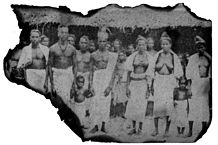
\includegraphics[width=\textwidth,height=8cm]{Kulasthree_Chapter_five_pic04.jpg}
\end{center}
\caption*{വാലസമുദായക്കാരുടെ വിവാഹസംഘം - കെ പി പത്മനാഭ മേനോൻ - വാള്യം 3 (1929), 1984}
\end{figure}

\paragraph{}പുടമുറി ഒഴിച്ചുള്ള മറ്റെല്ലാത്തരം വിവാഹരീതികളെയും അമർച്ചചെയ്യാനുള്ള പരിശ്രമമാണ് സമുദായപരിഷ്ക്കർത്താക്കളിൽനിന്നുണ്ടയത്. ഒരു സ്ത്രീക്ക് സ്വന്തം ജീവിതകാലത്ത് ഒരു ഭർത്താവിലധികം ഉണ്ടാകുന്നത് 'കുറച്ചി'ലാണെന്ന ധാരണ ക്രമത്തിൽ വളർന്നുവന്ന കാലവുംകൂടിയായിരുന്നു ഇത്. ഫാസറ്റ് അടക്കമുള്ള നിരവധി വിദേശികളും ചന്തുമേനോനെപ്പോലുള്ള സ്വദേശികളും ഇത്തരം നിലപാടുകളെ എതിർക്കാൻ ശ്രമിച്ചു. എന്നാൽ സമുദായപരിഷ്ക്കർത്താക്കളിൽ പലർക്കും ഇത് 'പുരുഷത്വം വീണ്ടെടുക്കലി'ന്റെ പ്രശ്നമായിരുന്നു. മരുമക്കത്തായത്തെ പൂർണ്ണമായും എതിർക്കാത്ത സമുദായമേധാവികൾപോലും അങ്ങനെ ചിന്തിച്ചു. 1909ൽ കൊടുങ്ങല്ലൂർ കുഞ്ഞിക്കുട്ടൻ തമ്പുരാൻ എഴുതിയ ലേഖനത്തിൽ ഇതു വ്യക്തമായും കാണാം:

\begin{quotation}
യഥാർത്ഥത്തിൽ പുരുഷത്വമുള്ളവർ മേത്തരം മലയാളികളിൽ വളരെക്കുറഞ്ഞുതന്നെയാണു നിൽക്കുന്നത്... ഒരു കന്യകയെ സ്വന്തം ഭാര്യയാക്കി സ്വീകരിച്ചാൽ ആ പെൺകുട്ടിയെ ഭരിപ്പാൻപോലും ത്രാണിയുള്ളവരായ പുരുഷന്മാർ വളരെ കുറവാണെന്നുള്ളതു തീർച്ചതന്നെ. ഈ വകക്കാരിൽ ഭാര്യയുടെ പരിപൂർണ്ണഭരണം വിട്ടുകൊടുക്കാതെ സ്ത്രീകളുടെ തറവാട്ടുസ്വത്തിന്മേൽ അവർക്കവകാശം എന്നേക്കും നിലനിർത്തിക്കൊണ്ട് ഒരുവിധം തീറ്റിപ്പോറ്റി രക്ഷിക്കുന്നതിനിടയാക്കുന്ന മരുമക്കത്തായ സമ്പ്രദായം അഭിനന്ദനീയംതന്നെ. പക്ഷേ, ഈവക പുരുഷന്മാരെ ഇങ്ങനെ [ 106 ] നപുംസകപ്രായന്മാരാക്കിത്തീർക്കാൻ കാരണവും മരുമക്കത്തായംതന്നെയാണെന്നു ചിലർ പറയുമായിരിക്കും. വാസ്തവത്തിൽ അങ്ങനെയല്ല. മരുമക്കത്തായത്തിന്റെ യഥാർത്ഥമല്ലാത്ത നിർവ്വഹണവും അവിഭക്തകുടുംബത്തിന്റെ ദുർഭരണവും നവീനവിദ്യാഭ്യാസത്തിന്റെ വികടഗതിയും എല്ലാം കൂടിക്കലർന്ന് നിലതെറ്റിയതിനാൽ മലയാളികളുടെ ഇടയിൽ പൌരുഷം അല്ലെങ്കിൽ പുരുഷത്വം ക്ഷയിച്ചു... ഈ സ്ഥിതിക്കു ഭാര്യയേയും മക്കളേയും ഭരിപ്പാനുള്ള പ്രാപ്തി ഈ യുവാക്കളിൽ അധികപക്ഷം ആളുകൾക്കും കിട്ടാഞ്ഞാൽ അത്ഭുതമില്ലല്ലോ...
\flushright{('സ്ത്രീകളുടെ ആപത്ത്', ലക്ഷ്മീഭായി 5(5), 1909)}
\end{quotation}


\paragraph{}ഈ മനോഭാവം വ്യാപകമായിത്തുടങ്ങുന്നകാലത്താണ് വരവിലയും വളർന്നത്. 'യഥാർത്ഥ പുരുഷൻ' ഭാര്യയെ ഭരിക്കുന്നവനാണെങ്കിൽ അവരുടെ സ്വത്തുക്കൾ കൈകാര്യംചെയ്യാനുള്ള അധികാരവും അയാൾക്കുതന്നെ എന്ന വിചാരത്തോടെ വിവാഹവേളയിൽ വധുവിന്റെ സ്വത്തിനെക്കുറിച്ചുള്ള അന്വേഷണവും തുടങ്ങി. സർക്കാർജോലിക്കാർക്ക് 'ഡിമാന്റുകൾ' ഏറുകയുംചെയ്തു. 1925ൽ തിരുവിതാംകൂറിലെ നായർ കൂട്ടുകുടുംബങ്ങൾ ഭാഗംവയ്ക്കാൻ അനുവദിച്ച നായർബിൽ പാസായതോടുകൂടി ഭാര്യയ്ക്കു ലഭിക്കേണ്ട ഓഹരി 'സ്ത്രീധന'മായി ഭർതൃഗൃഹത്തിലേക്ക് ഒഴുകാനും തുടങ്ങി..

\paragraph{} 1931ലെ തിരുവിതാംകൂർ ജനസംഖ്യാകണക്കെടുപ്പു (സെൻസസ്) റിപ്പോർട്ടിൽ 'യോഗ്യത'യുള്ള പുരുഷന്മാർക്ക് വൻതുക നൽകി പെൺകുട്ടികളെ വിവാഹംകഴിപ്പിക്കുന്ന രീതി നായർ-ഈഴവ കുടുംബങ്ങളിൽ കണ്ടുതുടങ്ങിയെന്ന നിരീക്ഷണമുണ്ട്. എന്നാൽ ഇതിനു വളരെമുമ്പുതന്നെ, ഈ സമ്പ്രദായം ആദ്യം കണ്ടുതുടങ്ങിയ ഘട്ടംമുതൽക്കേ, ഇതിനെയും ഇതിന്റെ സംരക്ഷകരായ സമുദായനേതാക്കന്മാരെയും കഠിനമായി വിമർശിച്ചവരുണ്ടായിരുന്നു. നായർ-ക്രിസ്ത്യൻ വിഭാഗങ്ങളിൽനിന്ന് ആധുനികവിദ്യാഭ്യാസം ചെയ്ത ആദ്യതലമുറക്കാരികൾ പലരും വരവിലയെ നിശിതമായി വിമർശിച്ചു. അവരിലൊരാളായിരുന്ന കെ. പത്മാവതി അമ്മ 1912ൽത്തന്നെ 'പണമെത്ര തരും?' എന്ന ചോദ്യവുമായി എത്തുന്ന സംബന്ധാന്വേഷകരെ നാല് ഇനമായി തിരിച്ചു. ആദ്യത്തേത് 'ശുദ്ധനാടൻ', അത് നാലാംക്ലാസ്സുകാർ. രണ്ടാമത്തേത്, അൽപ്പസ്വൽപ്പം ഇംഗ്ലീഷറിയും, ഒരു ചെറിയ ജോലിയുണ്ട് - അത് മൂന്നാം ക്ലാസ്സ്. നാലാം ക്ലാസ്സുകാരുടെ റേറ്റ് 200-500 രൂപയായിരിക്കുമ്പോൾ, മൂന്നാംക്ലാസ്സുകാരുടെ റേറ്റ് ആയിരമോ അതിനപ്പുറമോ ആയിരിക്കും. ബി.ഏ പാസായവരാണ് പിന്നെ രണ്ടാംക്ലാസ്സുകാർ. ആയിരത്തിനുമേലാണ് അവരുടെ റേറ്റ്. ഇവരുടെ ഉപരിപഠനം പലപ്പോഴും വധുവിന്റെ ചെലവിലാണ്. ഏറ്റവും മുകളിൽ ഒന്നാംക്ലാസ്സുകാരാണ്. അവർ സർക്കാരിന്റെ വകുപ്പുകളിൽ ഉദ്യോഗസ്ഥന്മാരോ വക്കീലന്മാരോ ഒക്കെയാണ്. ഇവരെക്കുറിച്ച് 'സാമാന്യക്കാരൊന്നും ഇവരുടെ കാര്യത്തെപ്പറ്റി ആലോചിക്കുകയേ വേണ്ട' എന്നാണ് പത്മാവതി അമ്മ പറയുന്നത്!

\paragraph{}

ഈ വില തീർച്ചപ്പെടുത്തലും കൊടുക്കലും കഴിയുമ്പോൾ കച്ചവടത്തിന്റെ യുക്തിയനുസരിച്ച് എല്ലാവരും ചിന്തിച്ചുതുടങ്ങുന്നതെങ്ങനെ എന്നവർ വിശദീകരിക്കുന്നു; സ്ത്രീകൾക്ക് അത് പ്രതികൂലമാകുന്നതെങ്ങനെ എന്നും:

\begin{quotation}
... പ്രിയസഹോദരിമാരെ! അല്പം ആലോചിച്ചാൽ നിങ്ങൾക്കുതന്നെ അറിവാൻ കഴിയും. വിലകൊടുത്തു വാങ്ങിയ ഒരു സാധനത്തിലോ അതല്ല വെറുതെ കിട്ടിയ ഒരു സാധനത്തിലോ നിങ്ങൾക്ക് അധികം പ്രിയമുണ്ടായിരിക്കുക? എന്തിനെയാണ് നിങ്ങൾ അധികം കരുതലോടും ശ്രദ്ധയോടുംകൂടി സൂക്ഷിക്കുകയും ശുശ്രൂഷിക്കുകയും ചെയ്യുക? വിലയ്ക്കുവാങ്ങിയ സാധനം നിങ്ങളുടെ ദൃഷ്ടിയിൽ പ്രത്യേകം പ്രിയമുള്ളതായും അതിനെ യാതൊരു കേടുപാടുംകൂടാതെ സൂക്ഷിക്കുന്നതിൽ നിങ്ങൾ അതീവനിഷ്ക്കർഷതയുള്ളവരുമായിരിക്കയില്ലെ? പുരുഷന്മാർ നിങ്ങളിൽനിന്നും മുഖ്യമായി ആവശ്യപ്പെടുന്നത് ഇതുതന്നെയാണ്... പണംകൊടുത്ത് ഒരു ഭർത്താവിനെ സമ്പാദിച്ചാൽ അദ്ദേഹത്തെ വേണ്ടപോലെ സൂക്ഷിക്കേണ്ടുന്ന ഭാരം ആർക്കാണെന്ന് ആലോചിച്ചു നോക്കുവിൻ... ഭർത്താവുംപോയി ചെലവുചെയ്ത പണവുംപോയി എന്നുള്ള നഷ്ടം സഹിക്കാതെ കഴിച്ചുകൂട്ടേണ്ടുന്ന ഭാരം ഭാര്യയ്ക്കാണ്...
\flushright{('പരിഷ്കൃതരീതിയിലുള്ള മലയാളി വിവാഹം', ലക്ഷ്മീഭായി 9(7), 1912)}
\end{quotation}

\paragraph{}വിവാഹം ഇത്രയും ചെലവുള്ള കാര്യമാകുമ്പോൾ വിവാഹമോചനത്തിന് സ്ത്രീകൾ മടിക്കും; പുനർവിവാഹത്തെക്കുറിച്ച് ആലോചിക്കാൻതന്നെ ഭയപ്പെടും! ഒരിക്കൽ വിവാഹമോചനം നേടിയ സ്ത്രീ രണ്ടാമതു വിവാഹംകഴിക്കാൻ ശ്രമിക്കുമ്പോൾ കൂടിയ വിലകൊടുക്കേണ്ടിവരും, കാരണം ഒരിക്കലവൾ വിവാഹംകഴിച്ചുവെന്ന കാര്യം അവളുടെ 'യോഗ്യതക്കുറവാ'യിട്ടാണ് നാട്ടിൽ എണ്ണുന്നത്! അവസാനമായി, 'യോഗ്യതയുള്ള' ഭർത്താവിനെ വിലയ്ക്കെടുക്കണമെങ്കിൽ കുടുംബസ്വത്തു പോര, സ്വകാര്യസ്വത്തുതന്നെ വേണമെന്ന് പത്മാവതി അമ്മ ഓർമ്മിപ്പിക്കുന്നു. കുടുംബസ്വത്താകുമ്പോൾ പൊതു ഉടമസ്ഥതയാണ്; സ്വകാര്യസ്വത്താണെങ്കിലേ അത് ചെറുക്കൻവീട്ടുകാർക്ക് കൈമാറാനൊക്കൂ. പെണ്ണിന്റെ യോഗ്യതയ്ക്ക് അത്ര വിലയൊന്നുമില്ല: 'പണം റൊക്കം കൊടുക്കാൻ ഒരുക്കമുണ്ടെങ്കിൽ എല്ലാം ഗുണപ്പെടും; ഇല്ലെങ്കിൽ ഒക്കെ ഗ്രഹപ്പിഴതന്നെ'

\paragraph{}ക്രിസ്ത്യാനികളുടെയിടയിലും ഇതേകാലത്താണ് സ്ത്രീധനത്തുക ക്രമാതീതമായി വർദ്ധിച്ചതും അനിയന്ത്രിതമായിത്തീർന്നതും. 1930കൾ ആയപ്പോഴേക്കും 'സാമ്പത്തിക കുഴപ്പത്തിന്റെ' നീരാളിപ്പിടുത്തംമൂലം കൃഷിയെ ആശ്രയിച്ചുജീവിച്ച കുടുംബങ്ങൾ വല്ലാത്ത പ്രതിസന്ധിയിലായി. 

\paragraph{}സ്ഥിരവരുമാനമുള്ള വരന്റെ വില കുതിച്ചുയരുകയുംചെയ്തു. പല സ്ത്രീകളും വിവാഹം വേണ്ടെന്നുവച്ച് ഉന്നതവിദ്യാഭ്യാസംനേടി ഉദ്യോഗസ്ഥകളും അദ്ധ്യാപികമാരും മറ്റുമായി. പരമ്പരാഗതകുടുംബങ്ങളിൽ വരവില ഉണ്ടാക്കിയ നഷ്ടത്തിന്റെയും വേദനകളുടെയും ഏറ്റവും മിഴിവുറ്റ ചിത്രങ്ങൾ 1940കളിലും 1950കളിലും ചെറുകഥകളെഴുതി പ്രസിദ്ധീകരിച്ച കെ. സരസ്വതിയമ്മയുടെ രചനകളിലാണുള്ളത്. (കാണുക \ref{saraswathy})

\paragraph{}
 സുറിയാനി ക്രിസ്ത്യാനികളിൽ പലരും വരവിലയുടെ വരവുകൊണ്ടുള്ള അപകടം നേരത്തെ തിരിച്ചറിയുകയും അതിനെതിരെ നിലപാടെടുക്കുകയും ചെയ്തിരുന്നു. സി.അന്തപ്പായി, കൊച്ചീപ്പൻ തരകൻ മുതലായ സമുദായസ്നേഹികൾ സ്ത്രീധനത്തിന്റെ അധഃപതനത്തെ എതിർക്കുകയും ആണ്മക്കളെ വിറ്റുകാശാക്കുന്ന കുടുംബക്കാരെ സമുദായത്തിനു പുറത്താക്കണമെന്ന് ആവശ്യപ്പെടുകയും ചെയ്തു. 1927ൽ ശ്രീമതി ഐ.സി. ചാക്കോ ഇങ്ങനെയെഴുതി:

\begin{quotation}
...ഒരാൾ കുറേ പണംകൊടുത്ത് ഒരു കാളയെയോ കുതിരയെയോ വിലയ്ക്കുവാങ്ങിക്കുന്നതുപോലെ ഒരു പിതാവ് തന്റെ പുത്രിക്ക് ഒരു വരനെ അവന്റെ യോഗ്യതാനുസരണം കൂടുതലായോ കുറവായോ ഉള്ള ഒരു വില അവന്റെ പിതാവിനു കൊടുത്തു വാങ്ങിക്കുന്നു. ആ വിലയാണ് നമ്മുടെ സ്ത്രീധനം. ആ ധനം ഭർത്താവിന്റെ പിതാവ് അയാളുടെ സ്വന്തംപോലെ ഉപയോഗിക്കുന്നു. സ്ത്രീ അതു കണികാണുകപോലും ചെയ്യുന്നില്ല. ഈ ഏർപ്പാടിനെ എത്ര പഴിച്ചാലും മതിയാവകയില്ല. ഇങ്ങനെ പുത്രന്മാരെ വിറ്റു ചെലവുകഴിക്കുന്ന മാതാപിതാക്കന്മാരുടെയും ഒരു സ്ത്രീയെ വിവാഹം കഴിക്കുന്നതിന് അവളുടെ പിതാവിനോടു സ്ത്രീധനമെന്നുപറഞ്ഞു കൈക്കൂലിവാങ്ങിക്കുന്ന ഭർത്താക്കന്മാരുടേയും പേരുകൾ... പത്രങ്ങളിൽ പ്രസിദ്ധപ്പെടുത്തി അവരുമായി സമുദായനിസ്സഹകരണമനുഷ്ഠിക്കുന്നത് ഇതിനൊരു പ്രതിവിധിയായിരിക്കുമെന്ന് തോന്നുന്നു.
\flushright{('നമ്മുടെ സ്ത്രീകൾ', വനിതാകുസുമം 1(6) 1927)}
\end{quotation}

\captionof{mybox}{1930കളിലെ സാമ്പത്തികമാന്ദ്യം}
\label{ch5box5} % place the caption
\begin{tcolorbox}[%
 breakable, % make the box breakable
  arc=0mm, 
  left=1pt, right = 1pt, 
  boxrule=0mm,
  colback = {blue!10}, % since shadow-gray was not defined
] 

\begin{center}
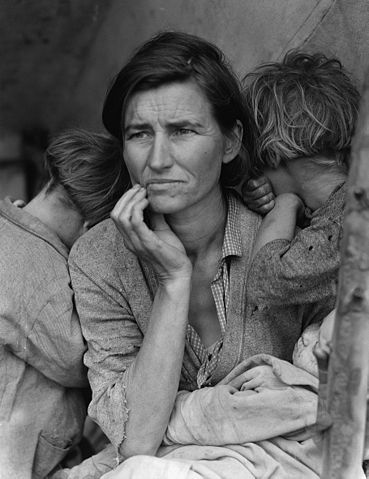
\includegraphics{Kulasthree_Chapter_five_pic05.jpg}
\end{center}


1920കളോടെ കേരളത്തിന്റെ സാമ്പത്തികവ്യവസ്ഥ വലിയ ഒരളവുവരെ ലോകവിപണിയുടെ ഭാഗമായിക്കഴിഞ്ഞിരുന്നു. വാണിജ്യവിളകൾ വ്യാപകമാവുകയും പണമിടപാട് സാധാരണമാവുകയും ചെയ്തു. തെങ്ങുകൃഷി 1900നുശേഷം വളരെ വിപുലമായിത്തീർന്നു; അക്കാലത്ത് തേങ്ങയ്ക്കു നല്ല വിലകിട്ടുകയും ചെയ്തു. പക്ഷേ, 1920കളുടെ ഒടുക്കം ലോകവിപണിയെ മുഴുവൻ ബാധിച്ച ഒരു വൻസാമ്പത്തികമാന്ദ്യം (Great Depression) പൊട്ടിപ്പുറപ്പെട്ടതോടെ നെല്ലിനും തേങ്ങയ്ക്കും വല്ലാതെ വിലയിടിഞ്ഞു. ചെറുകിടകർഷകരുടെ നട്ടെല്ലൊടിക്കുന്ന ഇടിവായിരുന്നു ഇത്. മരുമക്കത്തായകൂട്ടുകുടുംബങ്ങൾ ഭാഗംവയ്ക്കാൻ അനുവദിച്ച നിയമം തിരുവിതാംകൂറിൽ 1925ൽ നടപ്പിലായതിനുപുറകെയായിരുന്നു ഈ ആഘാതം. 1925നും 1931നുമിടയ്ക്ക് 33,000 ഭാഗപത്രങ്ങളാണ് തിരുവിതാംകൂറിൽ രജിസ്റ്റർ ചെയ്യപ്പെട്ടത്! കൃഷി ഗുണകരമല്ലെന്നുംകൂടിവന്നപ്പോൾ സ്വത്തുക്കളുടെ വില്പനയും വർദ്ധിച്ചു. കരത്തിലും സ്കൂൾഫീസിലുംമറ്റും തിരുവിതാംകൂർ സർക്കാർ ഇളവുകൾ പ്രഖ്യാപിച്ചെങ്കിലും ഭൂനികുതി അടയ്ക്കാൻ നിവൃത്തിയില്ലാതെ പുരയിടം വിറ്റവരുടെ എണ്ണം ക്രമാതീതമായി വർദ്ധിച്ചു. മലബാറിലാണെങ്കിൽ, ഭൂനികുതിയിലുണ്ടായ വർദ്ധനവ് ജനങ്ങളെ ദുരിതത്തിലാഴ്ത്തി; കൊച്ചിയിലും പണയഭൂമികളുടെ എണ്ണം വർദ്ധിക്കുകയും വാങ്ങാനാളില്ലാതെ കെട്ടിക്കിടക്കുകയും ചെയ്തു.
\end{tcolorbox}
 
 \begin{quotation}

പതിനഞ്ചാംവയസ്സിലായിരുന്നു എന്റെ വിവാഹം (1935ൽ). ഞങ്ങൾ പാവപ്പെട്ടവരായിരുന്നു; വരനും വരന്റെ വീട്ടുകാരും അങ്ങനെതന്നെ. എന്റെവീട്ടിൽവച്ചായിരുന്നു കല്യാണം. എനിക്ക് ഒരു കോടിവാങ്ങി; സമ്മാനങ്ങളോ സ്വർണ്ണോ ഒന്നും ഇല്ലായിരുന്നു. കുറച്ചു പൂവും പിന്നെ കറുത്ത ചരടിൽക്കോർത്ത താലിയുംമാത്രം. അന്നൊക്കെ നമ്മുടെയിടയിൽ ആർക്കും സ്വർണ്ണമാലയൊന്നും ഇല്ലായിരുന്നു. ഇന്നത്തെ ചെറുപ്പക്കാരികൾക്ക് ഇതു കൂടിയേതീരൂ... സ്ത്രീധനമെന്ന ഏർപ്പാടേ ഇല്ലായിരുന്നു. വളരെപ്പണ്ട് ചെറുക്കൻവീട്ടുകാർ പെൺവീട്ടുകാർക്ക് കല്യാണസമയത്ത് ചെറിയൊരു തുക കൊടുക്കുമായിരുന്നു. ഇത് ഇപ്പോഴില്ല... എന്റെ അമ്മയ്ക്ക് അതറിയുമായിരുന്നു. അമ്മയെ കല്യാണംകഴിച്ചപ്പോൾ അമ്മയുടെ അച്ഛന് ആ തുക കിട്ടിയത്രെ. ഇന്നാണെങ്കിൽ നേരെതിരിഞ്ഞു, നമ്മൾ ചെറുക്കൻ വീട്ടുകാർക്ക് വലിയതുക സ്ത്രീധനമായിക്കൊടുക്കുന്നു.
\flushright{(Anna Lindberg, Experience and Identity, 2001, പുറം 286-87).}
\end{quotation}
\captionof{mybox}{നിധീരിക്കൽ മറിയം അഥവാ ശ്രീമതി ഐ.സി. ചാക്കോ}
\label{ch5box6} % place the caption
\begin{tcolorbox}[%
 breakable, % make the box breakable
  arc=0mm, 
  left=1pt, right = 1pt, 
  boxrule=0mm,
  colback = {blue!10}, % since shadow-gray was not defined
] 


വിവാഹത്തിനുശേഷം ശ്രീമതി ഐ.സി ചാക്കോ എന്നിറിയപ്പെട്ട മറിയം, ആലപ്പുഴയിലെ അഭിജാതകുടുംബമായിരുന്ന നിധീരിക്കൽവീട്ടിൽ ജനിച്ചു. തിരുവനന്തപുരത്ത് വിദ്യാഭ്യാസത്തിനുശേഷം പതിനേഴാംവയസ്സിൽ സമുന്നത ശാസ്ത്രപണ്ഡിതനും ഗവേഷകനും സമുദായപ്രമാണിയുമായിരുന്ന ഐ.സി. ചാക്കോയെ വിവാഹം കഴിച്ചു. അനുജത്തിമാരായ തെരേസ നിധീരി, അന്നാ നിധീരി എന്നിവർ അദ്ധ്യാപികമാരെന്ന നിലയിൽ പ്രശസ്തരായെങ്കിലും മറിയം വിദ്യാഭ്യാസം തുടർന്നില്ല. 1930കളിൽ ക്രിസ്തീയവനിതകൾക്കുവേണ്ടി ശബ്ദമുയർത്തിയ സ്ത്രീയെന്ന നിലയിൽ പ്രസിദ്ധയായിരുന്നു.

\end{tcolorbox}

\paragraph{}1990കളായപ്പോഴേക്കും കീഴാളസമുദായസ്ത്രീകൾക്കിടയിൽ വിവാഹത്തെക്കുറിച്ചും സ്ത്രീത്വത്തെക്കുറിച്ചുമുള്ള മേലാളസങ്കല്പങ്ങൾക്ക് നല്ല വേരോട്ടമുണ്ടായിക്കഴിഞ്ഞുവെന്ന് ഈ ചരിത്രകാരി നിരീക്ഷിക്കുന്നു. നല്ല തുകകൊടുത്ത് 'യോഗ്യത'യുള്ള പുരുഷനെക്കൊണ്ടു വിവാഹം കഴിപ്പിക്കുന്നതാണ് പെണ്മക്കളുടെ സുരക്ഷിതത്വം ഉറപ്പിക്കാനുള്ള നല്ല മാർഗ്ഗമെന്ന് വിചാരിക്കുന്നതുകൊണ്ട് വർഷങ്ങളോളം ഫാക്ടറിയിൽ പണിയെടുത്തുകിട്ടിയ ആനുകൂല്യങ്ങൾപോലും പെണ്മക്കൾക്കു സ്ത്രീധനമായി കൊടുക്കാൻ അവർ തയ്യാറാണ്. എന്നാൽ ഇതുകൊണ്ട് ആ പെൺകുട്ടികൾ സുരക്ഷിതരാകുന്നുണ്ടോ? ഇല്ല എന്നതാണ് ദുഃഖസത്യം. ഇത്രയും വരവില കൊടുക്കുന്നുണ്ടെങ്കിലും, കശുവണ്ടിമേഖലയിലെ സ്ത്രീകളുടെ വിവാഹം പലപ്പോഴും അസ്ഥിരമാണ്. വരവിലയുടെ പേരുപറഞ്ഞാണ് ഇവിടെ പല ഭർത്താക്കന്മാരും ഭാര്യമാരെ ഉപേക്ഷിക്കുന്നത്!
\section{എന്തുകൊണ്ട് ഇങ്ങനെ സംഭവിച്ചു?}
\label{ch5sec3}

\paragraph{}20-ാം നൂറ്റാണ്ടിലെ കേരളത്തിൽ വരവില വിജയിച്ചുമുന്നേറിയതിന്റെ ചിത്രമാണ് ഇതുവരെ വരച്ചിട്ടത്. എന്തുകൊണ്ടിങ്ങനെ സംഭവിച്ചു എന്ന ചോദ്യം തീർച്ചയായും പ്രസക്തമാണ്. 'ഓഹരിമാത്രം മതി' എന്നു പറയുന്നവരും വധുവിന്റെ സ്വത്ത് കൈകാര്യംചെയ്യേണ്ടത് ഭർത്തൃകുടുംബമോ ഭർത്താവോ ആണ് എന്ന പൊതുസമ്മതത്തെ ആശ്രയിക്കുന്നവർതന്നെ. അതുപോലെ സ്ത്രീയെ പരിപാലിക്കാനുള്ള ചെലവാണ് സ്ത്രീധനമെന്നു പറയുന്നവരുണ്ട്; പക്ഷേ, 'പരിപാലനം' ആവശ്യമില്ലാത്ത, നല്ല ജോലിയും വരുമാനവുമുള്ള, സ്ത്രീകൾവരെ വരവില കൊടുക്കുന്നുണ്ട്. ഗൾഫ്നാടുകളിലും മറ്റുപലയിടത്തും ജോലിചെയ്ത് നന്നായി പണമുണ്ടാക്കുന്ന മലയാളിസ്ത്രീകളിൽ വലിയൊരുശതമാനം നേരിട്ടോ അല്ലാതെയോ വരവില നൽകുന്നവരാണ്.

\paragraph{}ഈ വിഷയത്തെക്കുറിച്ച് കൂടുതൽ പഠനങ്ങൾ ഉണ്ടാകേണ്ടതാണ്; ചില കാര്യങ്ങൾ ചർച്ചയ്ക്കായി ഇവിടെ സൂചിപ്പിക്കുന്നെന്നുമാത്രം. തീർച്ചയായും വരവിലയുടെ വളർച്ചയെ കേരളത്തിൽ 19-ാം നൂറ്റാണ്ടിനുശേഷം വളർന്നുവന്ന മുതലാളിത്തവ്യവസ്ഥയുമായി ബന്ധപ്പെടുത്തണം. മുതലാളിത്തവ്യവസ്ഥയിൽ സ്വത്തുക്കൾ സ്വകാര്യമായി സമ്പാദിക്കാനുള്ള സാദ്ധ്യത വളരെ വർദ്ധിച്ചുവെന്നുമാത്രമല്ല, ജീവിതത്തിന്റെ സമസ്തമേഖലകളിലും കച്ചവടം, ലാഭം എന്നിവയുടെ കണക്കുകൂട്ടൽ അധികമായി. കുടുംബം 'പരിപാവന'മാണ്, 'എല്ലാക്കാലത്തും നിലനിൽക്കുന്ന'താണ് എന്നൊക്കെ നാം പറയുമെങ്കിലും, ആ സ്ഥാപനവും ഈ മുതലാളിത്തമൂല്യങ്ങൾക്ക് കീഴ്പ്പെട്ടാണ് നിൽക്കുന്നത്. അവിടെയുള്ള ബന്ധങ്ങളും കച്ചവടയുക്തിക്കു കീഴ്വഴങ്ങി - സ്ത്രീകൾക്ക് അനുകൂലമായ രീതിയിലല്ലെന്നുമാത്രം. ആൺകോയ്മയും കച്ചവടയുക്തിയും ഒന്നിച്ചുകൂടുന്നിടത്ത് വരവിലപോലുള്ള സ്ത്രീവിരുദ്ധസ്ഥാപനങ്ങൾ തഴച്ചുവളരുകതന്നെചെയ്യും. 20-ാം നൂറ്റാണ്ടിലെ സമുദായനവീകരണപ്രസ്ഥാനങ്ങളുടെ താത്പര്യങ്ങളും പുരോഗമനപ്രസ്ഥാനങ്ങളുടെ വീഴ്ചകളും കണ്ടില്ലെന്നു നടിച്ചുകൂടാ. സമുദായപ്രസ്ഥാനങ്ങൾ പൊതുവെ അണുകുടംബത്തെ (അതായത്, ഭാര്യാഭർത്താക്കന്മാരും കുട്ടികളുമടങ്ങിയ കുടുംബം) സമുദായത്തിന്റെ ഉറച്ച അടിസ്ഥാനഘടകമായി കണക്കാക്കുകയും, അതു സംരക്ഷിക്കപ്പെടേണ്ടതാണെന്ന് ഊന്നിപ്പറയുകയും ചെയ്തു. ഈ പുതിയ കുടുംബത്തിലും സ്ത്രീ മിക്കപ്പോഴും രണ്ടാംതരക്കാരിയായിപ്പോകുന്നു എന്ന് ആദ്യകാലസ്ത്രീപക്ഷവാദികൾ ചൂണ്ടിക്കാണിക്കാൻ ശ്രമിച്ചിരുന്നു - കെ. പത്മാവതി അമ്മ അവരിൽ ഒരാൾ മാത്രമായിരുന്നു. പൊതുവെ ഈ പരാതികളെ 'കുടുംബദ്രോഹ'മോ 'സമുദായവിരോധ'മോ ആയാണ് സമുദായനേതാക്കന്മാർ എണ്ണിയത്. പഴയ കൂട്ടുകുടുംബങ്ങളായിരുന്നു നല്ലതെന്ന് ഈ സ്ത്രീകൾ ഒരിക്കലും പറഞ്ഞില്ല - പക്ഷേ, സമുദായനേതൃത്വങ്ങൾ ഉയർത്തിക്കാട്ടിയ പുതിയ കുടുംബമാതൃക സ്ത്രീയോട് നീതിപുലർത്തില്ലെന്ന് അവർ വിളിച്ചുപറഞ്ഞു. കുടുംബത്തെ 'ശാശ്വത'മെന്നും 'പാവന'മെന്നും എണ്ണി അതിനു കീഴ്വഴങ്ങാതെ കൂടുതൽ ജനാധിപത്യവൽക്കരണം ആവശ്യമുള്ള ഒരു സ്ഥാപനമാണതെന്ന് അവർ വാദിച്ചു. കുടുംബാംഗങ്ങൾക്കെല്ലാം തുല്യപരിഗണന നൽകുന്ന ഒരു സ്ഥാപനമായി കുടുംബത്തെ മാറ്റിയെടുക്കുന്നതിനെക്കുറിച്ചുള്ള ചർച്ച 1940കൾക്കുശേഷം വളരെ കുറച്ചുമാത്രമേ നടന്നിട്ടുള്ളുവെന്ന് പറയാം. വരവിലയുടെ പ്രശ്നം ഒരു പ്രശ്നമായി നാം തിരിച്ചറിയാൻ ഇത്ര വൈകിയത് ഇതുകൊണ്ടായിരിക്കാം. എന്നാൽ ഈ ചർച്ച തുടങ്ങിവയ്ക്കാൻ ശ്രമിക്കുന്നവരെ 'കുടുംബവിരോധി'കളെന്നോ 'സമുദായശത്രു'ക്കളെന്നെ മുദ്രകുത്തുന്ന രീതിയാണ് ഇന്നും നിലവിലുള്ളത്!

\paragraph{}

ഇതുകൂടാതെ മലയാളികളായ നാം പൊതുജീവിതത്തിന്റെ വിലയെ വല്ലാതെ കുറയ്ക്കുകയും കുടുംബജീവിതത്തെ കണക്കിലധികം വിലമതിക്കുകയും ചെയ്യുന്നില്ലേ എന്ന ചോദ്യവുമുണ്ട്. വിവാഹംകഴിക്കാത്ത ഒരു വ്യക്തിക്ക് പലതും ചെയ്യാം - ജീവിതകാലംമുഴുവൻ പൊതുപ്രവർത്തനത്തിലേർപ്പെടാം, സാമൂഹ്യസേവനം നടത്താം, സാഹിത്യ-കലാപ്രവർത്തനങ്ങളിൽ മുഴുകാം. പക്ഷേ, മലയാളികൾക്ക് വിവാഹവും ദാമ്പത്യജീവിതവും കഴിഞ്ഞേ ഇതൊക്കെയുള്ളൂ! വിവാഹം കഴിക്കാത്ത ഒരു വ്യക്തിക്ക് എന്തോ കുറവുണ്ടെന്ന് നാം വിചാരിക്കുന്നു; സ്വന്തംകാലിൽ നിൽക്കാനുള്ള വരുമാനമോ വേലയോ ഇല്ലാത്ത വ്യക്തിക്ക് നമ്മുടെ കണ്ണിൽ ഒരു കുഴപ്പവുമില്ല! ഈ കല്യാണം കഴിക്കാത്ത കക്ഷി ഒരു സ്ത്രീയാണെങ്കിൽ പറയുകയും വേണ്ട! 'രാഷ്ട്രീയപ്രബുദ്ധത'യ്ക്കു പേരുകേട്ട നാടാണല്ലോ കേരളം. പക്ഷേ, ഇവിടെ പൊതുജീവിതത്തിനല്ല, കുടുംബജീവിതത്തിനാണ് സർവ്വപ്രാധാന്യം! പൊതുപ്രവർത്തകരായ പുരുഷന്മാരുടെ ആത്മകഥകൾ പരിശോധിച്ചുനോക്കുക - അമ്മയുടെയും ഭാര്യയുടെയും ത്യാഗത്തെ വണങ്ങാൻ അവർ മറക്കാറില്ല. എന്നാൽ നിഷ്ക്രിയമായ ത്യാഗത്തിലുപരിയായി പൊതുപ്രവർത്തനത്തിൽ അമ്മയ്ക്കോ ഭാര്യയ്ക്കോ പങ്കില്ലെന്ന വസ്തുത അവരിലേറെപ്പേരെയും അധികം അലട്ടുന്നില്ല.
\paragraph{}1940കളിൽ - ഇവിടത്തെ കമ്മ്യൂണിസ്റ്റ്പ്രസ്ഥാനവും ദേശീയപ്രസ്ഥാനവും ഏറ്റവും ശക്തമായിരുന്ന ആ കാലത്ത് - ആദ്യകാലകമ്മ്യൂണിസ്റ്റ് പ്രവർത്തകരായിരുന്ന പല പ്രമുഖരും പൂർണ്ണമായ പൊതുജീവിതത്തിനുവേണ്ടി കൊതിച്ചതാണ്. സ്വന്തം വീട്, കൂട് എന്നിവയിൽ തങ്ങളുടെ പ്രതിബദ്ധത ഒതുങ്ങിപ്പോകരുതെന്ന് വാശിയുള്ള തലമുറയായിരുന്നു അത്. വിവാഹം, കുടുംബംവളർത്തൽ എന്ന ഒറ്റ ലക്ഷ്യമല്ല മനുഷ്യജന്മത്തിനുള്ളതെന്ന് അവർ കരുതി. സാമൂഹ്യപ്രവർത്തനത്തിലൂടെ, രാഷ്ട്രീയപ്രവർത്തനത്തിലൂടെ, പൊതുജനങ്ങൾക്കൊപ്പം പ്രവർത്തിക്കുന്നതിലൂടെ കുടുംബജീവിതത്തെക്കാളേറെ ധന്യമായ ജീവിതം സാദ്ധ്യമാണെന്നായിരുന്നു അവരുടെ പക്ഷം. പക്ഷേ, 1940കളിലെ രാഷ്ട്രീയപ്രതിസന്ധികൾ ശമിച്ചതോടെ ഇങ്ങനെ മറ്റുള്ളവരിൽനിന്ന് വ്യത്യസ്തമായ ജീവിതലക്ഷ്യത്തെ പിന്തുടരുന്ന രീതിയെ പ്രാത്സാഹിപ്പിക്കേണ്ടതില്ലെന്ന് കമ്മ്യൂണിസ്റ്റ് നേതൃത്വം തീരുമാനിച്ചു. മുഴുവൻസമയപ്രവർത്തകരായി രംഗത്തുവന്നവർ കുടുംബങ്ങളിലേക്കു മടങ്ങി അതിന്റെ പരിധികൾക്കുള്ളിൽനിന്നുകൊണ്ട് പ്രവർത്തിക്കണമെന്നായിരുന്നു നേതൃത്വത്തിന്റെ നിർദ്ദേശം. ഇ.എം.എസ് നമ്പൂതിരിപ്പാട് ഇക്കാര്യത്തിൽ കൈക്കൊണ്ട നിലപാട് അദ്ദേഹത്തിന്റെ 'പുതിയ ചട്ടങ്ങൾ' (1944) എന്ന ലേഖനത്തിൽനിന്നു വ്യക്തമാകുന്നുണ്ട്. (ഇ.എം.എസ് സമ്പൂർണ്ണകൃതികൾ, വാള്യം 5, തിരുവനന്തപുരം, 1999, പുറം 172-217) കമ്മ്യൂണിസ്റ്റ് രാഷ്ട്രീയപ്രവർത്തനത്തിലേർപ്പെട്ടിരുന്ന വനിതകൾക്കുപോലും സ്ത്രീധനസമ്പ്രദായത്തിൽനിന്ന് പൂർണ്ണമായും രക്ഷനേടാൻ കഴിഞ്ഞില്ല. (കാണുക \ref{ch11box13}).

\paragraph{}1940കളിലെ പരീക്ഷണങ്ങൾ മുന്നോട്ടുപോയിരുന്നെങ്കിൽ, ഒരുപക്ഷേ, കേരളത്തിൽ കുടുംബത്തിനും വിവാഹത്തിനും കൽപ്പിക്കുന്ന പ്രാധാന്യവും അതിനോടൊപ്പം വളരുന്ന വരവിലയും ഇത്രയുമാകില്ലായിരുന്നു. വിവാഹം വേണ്ടെന്നുവയ്ക്കുന്നവരും വിവാഹം നടക്കാതിരിക്കുന്നവരും ഇത്രയേറെ പരിഹാസത്തെയും സംശയത്തെയും നേരിടേണ്ടിവരില്ലായിരുന്നു. സ്വന്തം കുടുംബത്തിനപ്പുറം മനുഷ്യരുണ്ടെന്നും അവർക്കൊപ്പം നിൽക്കുന്നതാണ് ധന്യജീവിതമെന്നും വാദിക്കുന്നവരുടെ എണ്ണം ഇത്രയും കുറഞ്ഞുപോകില്ലായിരുന്നു!



\section{അവസാനവാക്ക്}
\label{ch5sec4}
ഈ അദ്ധ്യായത്തിന്റെ അവസാനവാക്ക് 1912ൽ വരവിലയ്ക്കു പരിഹാരം പെൺകുട്ടിയുടെ ആത്മാഭിമാനവും ജീവിതത്തിൽ പിടിച്ചുനിൽക്കാനുള്ള ധൈര്യവുമാണ് എന്നു തിരിച്ചറിഞ്ഞ ചെറുവാരി രുഗ്മിണിയമ്മയ്ക്കാണ്. കെ. പത്മാവതിയമ്മ ഇവരുടെ വാക്കുകളെ സ്വന്തം ലേഖനത്തിൽ കടമെടുത്ത് ഉപയോഗിച്ചു. അതുതന്നെ ഇവിടെയും ചെയ്യുന്നു:
\begin{quotation}
ഇച്ഛയ്ക്കും യോഗ്യതയ്ക്കും തക്കതായ വരനെ ലഭിക്കാത്തപക്ഷം തങ്ങളെ സർവ്വാരിഷ്ടങ്ങളിൽ [സർവ്വകഷ്ടപ്പാടുകളിൽ]നിന്നും ത്രാണനംചെയ്തു തീറ്റിപ്പോറ്റിയ മാതാപിതാക്കളുടെ ശുശ്രൂഷയെ ചെയ്തു പുണ്യം സമ്പാദിക്കുകയോ, അവരവരുടെ ബുദ്ധിശക്തിക്കും സൗകര്യത്തിനും അനുസരിച്ചതായ വിദ്യാഭ്യാസവും സമ്പാദിച്ച് അവസ്ഥാനുസരണമായ വല്ല ജോലികളിൽ ഏർപ്പെടുകയോ ചെയ്യുന്നതാണ് ശ്രേയസ്കരം... ഇപ്രകാരം സുഖാനുഭവത്തിനും ധർമ്മസമ്പാദനത്തിനും മോക്ഷത്തിനും പലേ പന്ഥാവുകളോടു [വഴികളോടു]കൂടിയ ഈ പ്രപഞ്ചത്തിൽ പത്നിത്വം [ഭാര്യാപദവി] ഒന്നുമാത്രമാണ് സ്ത്രീധർമ്മം എന്ന മൂഢവിശ്വാസത്തോടുകൂടി ആധിവ്യാധിദാരിദ്ര്യാദിപൂർണ്ണമായ [കഷ്ടപൂർണ്ണമായ] ഭവാംബുധിയിൽ [ലോകമാകുന്ന സാഗരത്തിൽ] മുഴുകി കരകാണാതെ ഉഴന്നു ജന്മം നശിപ്പിക്കുന്നത് മഹാപാതകമാകുന്നു.
\flushright{(ലക്ഷ്മീഭായിയിൽ 1912ൽ എഴുതിയ ഒരു ലേഖനത്തിൽനിന്ന് പത്മാവതിയമ്മ ഉദ്ധരിച്ച വാക്കുകൾ.)}

\end{quotation}

\section{കൂടുതൽ ആലോചനയ്ക്ക്}
\label{ch5sec5}
'കേരളീയനവോത്ഥാന'ത്തെക്കുറിച്ച് നിലവിലുള്ള പല ചരിത്രപുസ്തകങ്ങളും മുന്നോട്ടുവയ്ക്കുന്ന മനോഹരചിത്രത്തിന് അല്പം മങ്ങലേല്പിക്കുന്ന കാര്യങ്ങളാണ് ഈ അദ്ധ്യായത്തിൽ ചർച്ചചെയ്തത്. ചരിത്രരചനയുടെ രാഷ്ട്രീയത്തെക്കുറിച്ച് നാമെന്താണ് ഇതിൽനിന്ന് പഠിക്കുന്നത്? 'പുരോഗമനപരം' എന്ന് പൊതുവെ വാഴ്ത്തപ്പെടുന്ന സാമൂഹ്യമാറ്റങ്ങൾ സ്ത്രീപക്ഷത്തുനിന്നു പരിശോധിക്കുമ്പോൾ ലഭിക്കുന്നത് മറ്റൊരു ചിത്രമാണ്! 

\begin{center}
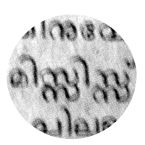
\includegraphics{Kulasthree_Chapter_five_pic06.jpg}
\end{center}
